\chapter{Machine Learning techniques} \label{chap3}
\section{Introduction}
In this chapter, we will focus on the more traditional methods used in natural language processing such as Na\"{i}ve-Bayes, decision trees, linear SVM and others. These will serve as a baseline for comparing the performances of the more two advanced models that will be analysed later on: LSTM and Attention Mechanism. The first thing to do when working with text is the do words and texts embedding, indeed, in order to use machine learning algorithms on texts, a mathematical representation of these texts is required. 
\section{Text to vectors}
As explained before, text needs to be represented in a way that gives more meaningful information than a simple sequence of bits, which have additional drawbacks such that for a given word, the sequence of bits representing it depends on the coding.
 The first and simplest coding that comes to mind is a one-hot encoding: a matrix $M$ of size number of texts $\times$ number of words where $M_{ij} = 1$ if the word $j$ is present in the text  $i$ and $0$ in the other case. But this is still not enough as each word is given the same weight, no matter how often it appears in the text. \\ 
 In order to overcome this problem, term-frequency might be used, that is, rather than setting $M_{ij}$ to 0 or 1 we set it to the amount of time it appears in the text. \\ 
 It is possible to use even better text embedding. It is called term-frequency, inverse document frequency. The main idea is that a word that appears often in all the documents is not helpful in order to classify the documents. For example, if the task is to classify books of biology and physics, words atoms, cells or light are more useful than today or tomorrow. \\
In order to compute tf-idf, it is separated in two parts, the first one being term frequency and the second one inverse document frequency. We have that \begin{equation}
 tf_{ij} = \#(W_j | W_j \in D_i)\\ 
\end{equation}
That it $tf_{ij}$ is the number of times the word j appears in the document i. 
Secondly, we have that \begin{equation*}
 idf_{j} = \log(\frac{\#D}{\#(D_i | W_j \in D_i)}) \\
\end{equation*}
this is the log of the total number of documents, over the number of documents that contains the word j.
Finally, the value tfidf value is computed by \begin{equation}
 tf-idf_{ij} = tf_{ij} * idf_{j} \\
\end{equation}
This the text embedding methods that will be used in this section. 
\section{Methodology}
\paragraph{} All the methods presented will be tested in two different ways: 
\begin{itemize}
 \item On the liar-liar dataset
 \item On the fake corpus dataset, excluding the news from \textit{beforeitsnews.com} and \textit{nytimes.com}
\end{itemize}
To be more precise, in the first case, the models will be trained on a training set, tuned using validation set and finally tested using test set. In the second case, the same methodology will be used, the dataset has been split be choosing $60\%$ of the text from each domain for training, and $20\%$ for validation and testing. This way of splitting has been chosen because of the uneven representation of each domain in the dataset in order to ensure representation of all the domains in the tree subsets. 
\subsection{Evaluation Metrics}
In order to evaluate each model, multiple evaluation metrics have been used. There are recall, precision and f1-score. It is needed to use multiple metrics because they don't all account for the same values. For instance, it is possible to have a model with a recall of 1 that behave extremely bad because it simply classifies all the inputs in the same single class. 
Remember That Precision Is Defined As \begin{equation}
 Precision = \frac{TP}{TP + FP}
\end{equation}
Which means that we can have two different precision, depending on which classes is considered as being positive. This is the proportion of correctly classified positive elements over the number of elements classified as positive. It is equals to 1 when there is no false positive, but it does not mean that all the positive elements are correctly classified as it might be some false negative. The recall helps to solve this problem.
It Is Defined As \begin{equation}
 recall = \frac{TP}{TP + FN}
\end{equation}
The f1-score combines the recall and the precision. It is defined by 
\begin{equation}
 f1-score = \frac{2 * precision * recall}{precision + recall}\
\end{equation}
It is also possible to look at the weighted average of all these values. For instance, it is possible to compute the global recall by averaging the recall for both classes by the respective class ratio. \\
Finally, raw output can be used by looking at the confusion matrix.\\
The first parameter to tune is the max number of features used by tf-idf. This is the maximum number of words that will be kept to create the text encoding. The words that are kept are the most frequent words. 
\section{Models}
Four models have been used in order to classify texts represented as a TF-IDF matrix. These are Multinomial Na\"{i}ve-Bayes, Linear SVM, Ridge Classifier and Decision Tree. I will start by a very brief recap of each model and how they work. 
\subsection{Na\"{i}ve-Bayes\cite{zhang_optimality_nodate}}
The basic idea of Na\"{i}ve-Bayes model is that all features are independent of each other. This is a particularly strong hypothesis in the case of text classification because it supposes that words are not related to each other. But it knows to work well given this hypothesis. 
Given an element of class y and vector of features $\mathbf{X} = (x_1,...,x_n)$. The probability of the class given that vector is defined as 
\begin{equation}
 P(y | \mathbf{X}) = \frac{P(y)*P(\mathbf{X} | y)}{P(\mathbf{X})}
\end{equation}
Thanks to the assumption of conditional independence, we have that 
\begin{equation}
 P(x_i |y,x_1, ...,x_{i-1},x_{i+1},...,x_n) = P(x_i | y)
\end{equation}
Using Bayes rules we have that
\begin{equation}
 P(y|x_1,...,x_n) = \frac{P(y)\prod_{i=1}^n P(x_i | y)}{P(x_1,...,x_n)}
\end{equation}
Because $P(x_1,...,x_n)$ is constant, we have the classification rule 
\begin{equation}
 \hat{y} = \underset{y}{argmax} P(y)\prod_{i=1}^n P(x_i | y)
\end{equation}
\subsection{Linear SVM}
Linear SVM is a method for large linear classification. Given pairs of features-label $(\mathbf{x_i}, y_i), y_i \in \{-1, 1\}$, it solves the following unconstrained optimization problem. 
\begin{equation}
 \underset{w}{min} \frac{1}{2} \mathbf{w^Tw} + \mathbf{C} \sum_{i=1}^l \xi(\mathbf{w;x_i},y_u)
\end{equation}
Where $\xi$ is a loss function, in this case L2 loss function has been used, and $\mathbf{C} > 0$ a penalty parameter. 
Class of new examples are assigned by looking at the value of $\mathbf{w^Tw}$. The class 1 is assigned if $\mathbf{w^Tw} \geq 0$ and the class $-1$ if $\mathbf{w^Tw} < 0$.
\subsection{Decision Tree\cite{Rokach:2014:DMD:2755359}}
Decision tree works by recursively selecting features and splitting the dataset on those features. These features can either be nominal or continuous. \\
In order to find the best split, it uses gini impurity. 
\begin{equation}
 G = \sum_{i=1}^C p(i) * (1-p(i))\\
\end{equation}
Where $p(i)$ is the probability of class i in the current branch. The best split is chosen as the one that decreases the most the impurity. For instance, beginning from the root, the gini impurity is computed on the complete dataset, then the impurity of each branch is computed over all features, weighting it by the number of elements in each branch. The chosen feature is the one that has the highest impurity. 
\subsection{Ridge Classifier}
Ridge classifier works the same way as ridge regression. It states the problem as a minimization of the sum of square errors with penalization. It can be expressed as in \textbf{Equation \ref{eq:ridge}}.
\begin{equation}
 \underset{w}{min} ||Xw-y||^2_2 + \alpha ||w||^2_2 \label{eq:ridge}
\end{equation}
The predicted class if positive if Xw is positive and negative otherwise. 
\section{Models on liar-liar dataset}
\subsection{Linear SVC}
In the case of linear SVC there is one parameter to tune up, which is the penalty parameters for the error term. \textbf{Figure \ref{fig:chap3:linearSVC}} shows the three main metrics with respect to the penalty parameter. This show that a parameter of around $0.1$ is the best one. 
\begin{figure*}[]
 \centering
 \makebox[\textwidth][c]{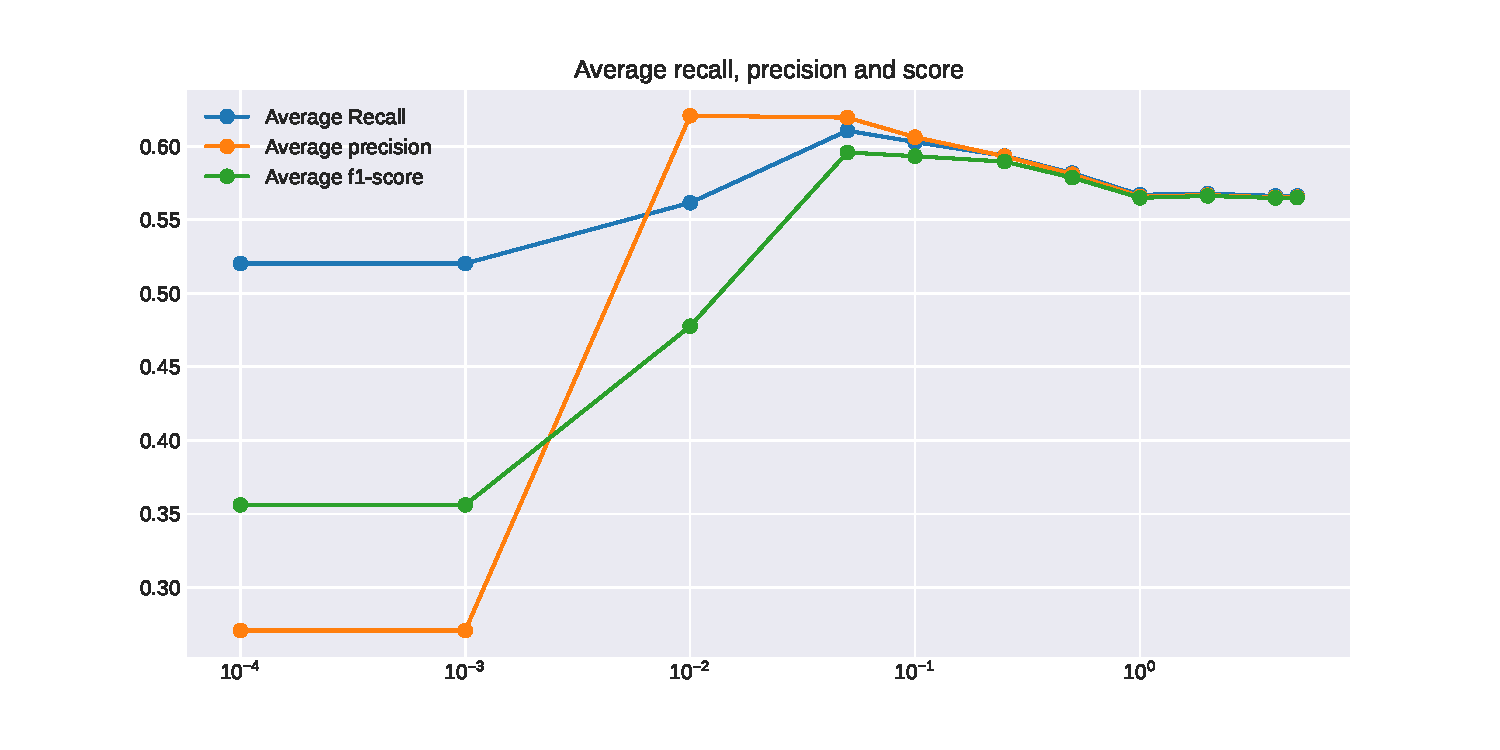
\includegraphics[width=1\textwidth]{images/chapitre3/svc_liar.pdf}}
 \caption{Tuning linearSVC parameters }
 \label{fig:chap3:linearSVC}
\end{figure*}
\subsection{Decision Tree}
With decision trees, it is possible to reduce overfitting by pruning the tree. It is possible to do pre-pruning or post pruning. Pre-pruning means that a stopping criterion is used to stop tree growth earlier and post pruning cut the tree once it has been fully grown. It this case pre-pruning is done by limiting the maximum depth of the tree. 
\begin{figure*}[]
 \centering
 \makebox[\textwidth][c]{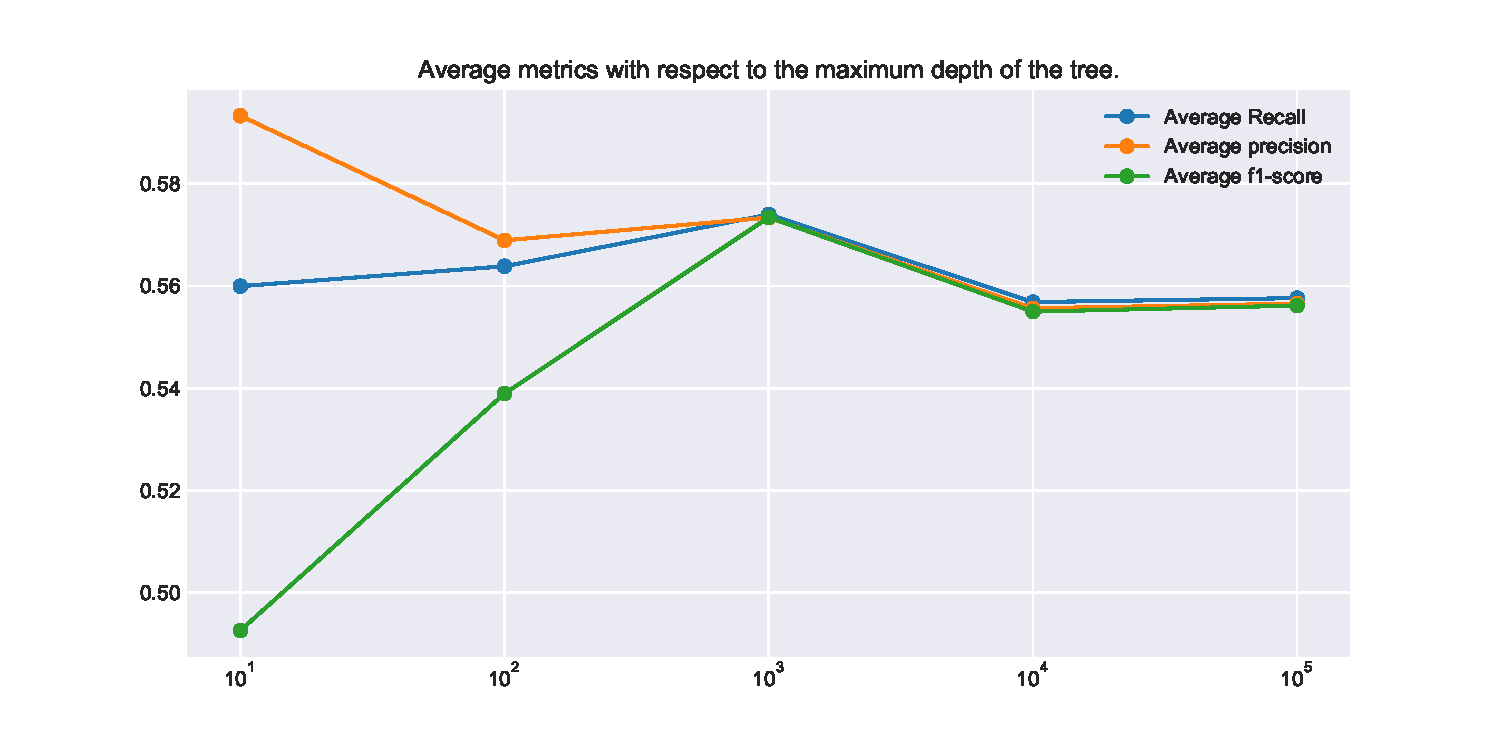
\includegraphics[width=1\textwidth]{images/chapitre3/liar-dt.pdf}}
 \caption{Tuning Decision Tree Parameters }
 \label{fig:chap3:dt}
\end{figure*}
\textbf{Figure \ref{fig:chap3:dt}} shows metrics values for different depths. It seems that tree of depth 1000 are the best ones.
\subsection{Ridge Classifier}
With the ridge classifier model, it is also possible to tweak the penalty value of the optimization problem. At \textbf{Figure \ref{fig:chap3:ridge1}} we can see that the optimal parameter is around 10 or 20, depending of the metrics that we want to maximize. Later on, the value of 10 will be chosen as a compromise between precision and recall. It is the value that maximizes the f1-score. 
\begin{figure*}
 \centering
 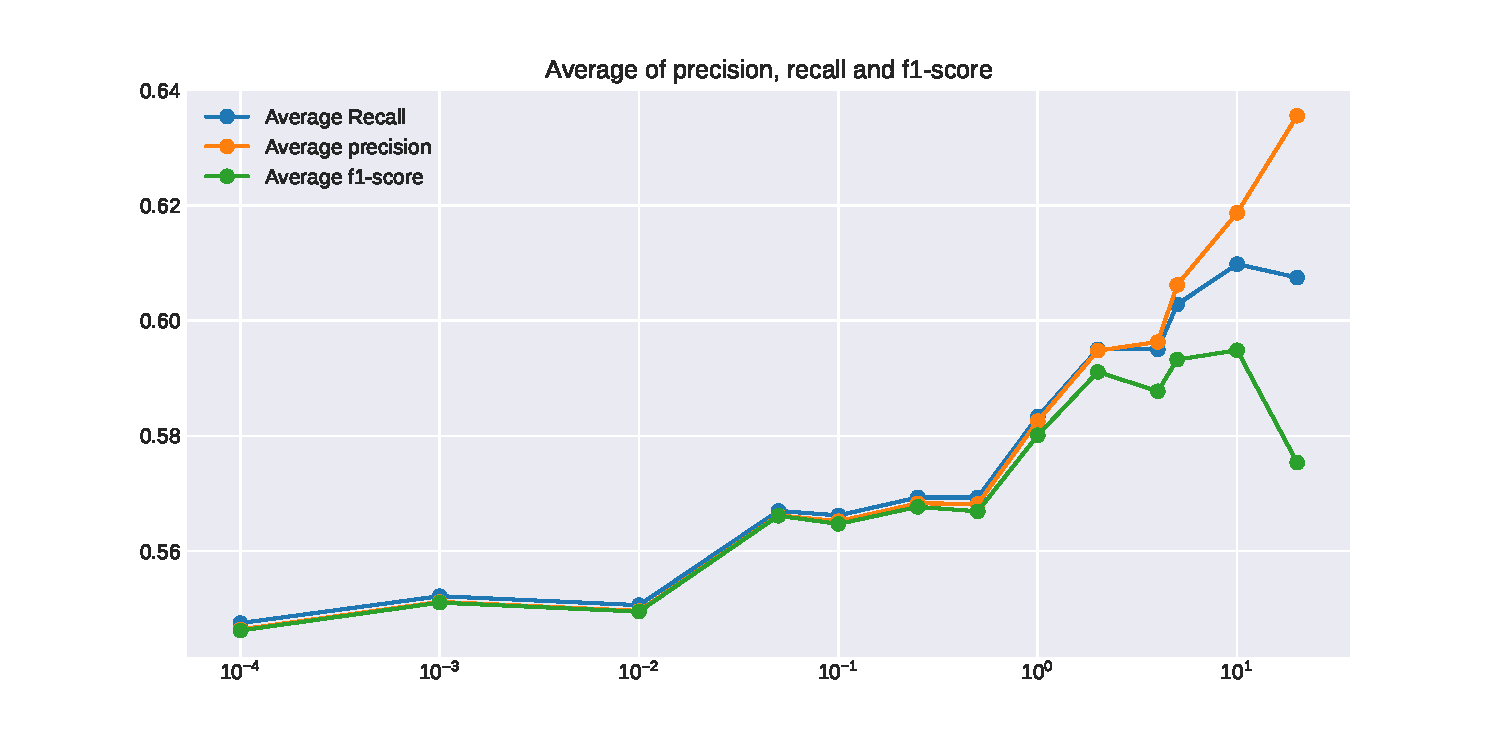
\includegraphics[width=1\textwidth]{images/chapitre3/liar-ridge}
 \caption{Average metrics for ridge classifiers with respect to the penalty parameter.}
 \label{fig:chap3:ridge1}
\end{figure*} 
\subsection{Max Feature Number}
Starting with the maximum number of features, the precision of each model can be analysed when limiting the maximum number of words. The results for each model can be seen at \textbf{Figure \ref{fig:chap3:max_feature3}, \ref{fig:chap3:max_feature1}} and \textbf{\ref{fig:chap3:max_feature2}}. Shows that depending on the metrics we want to optimize it is better to choose different parameters. For instance, in order to maximize F1-score, it is better to use a maximum number of features of 1000.\\
The results are slightly different if the goal is to optimize the precision because if the best value stays the same for Linear SVM and Ridge Classifier, the Na\"{i}ve-Bayes work better when using the maximum number of features and it goes the same way for recall. 
Based on \textbf{Figure \ref{fig:chap3:max_feature3}} we can say that when it comes to precision and recall, Na\"{i}ve-Bayes is the one that performs the best.\\
Row results for max features selection are available at \textbf{Appendix \ref{Appendix1}}.
\begin{figure*}[]
 \centering
 \makebox[\textwidth][c]{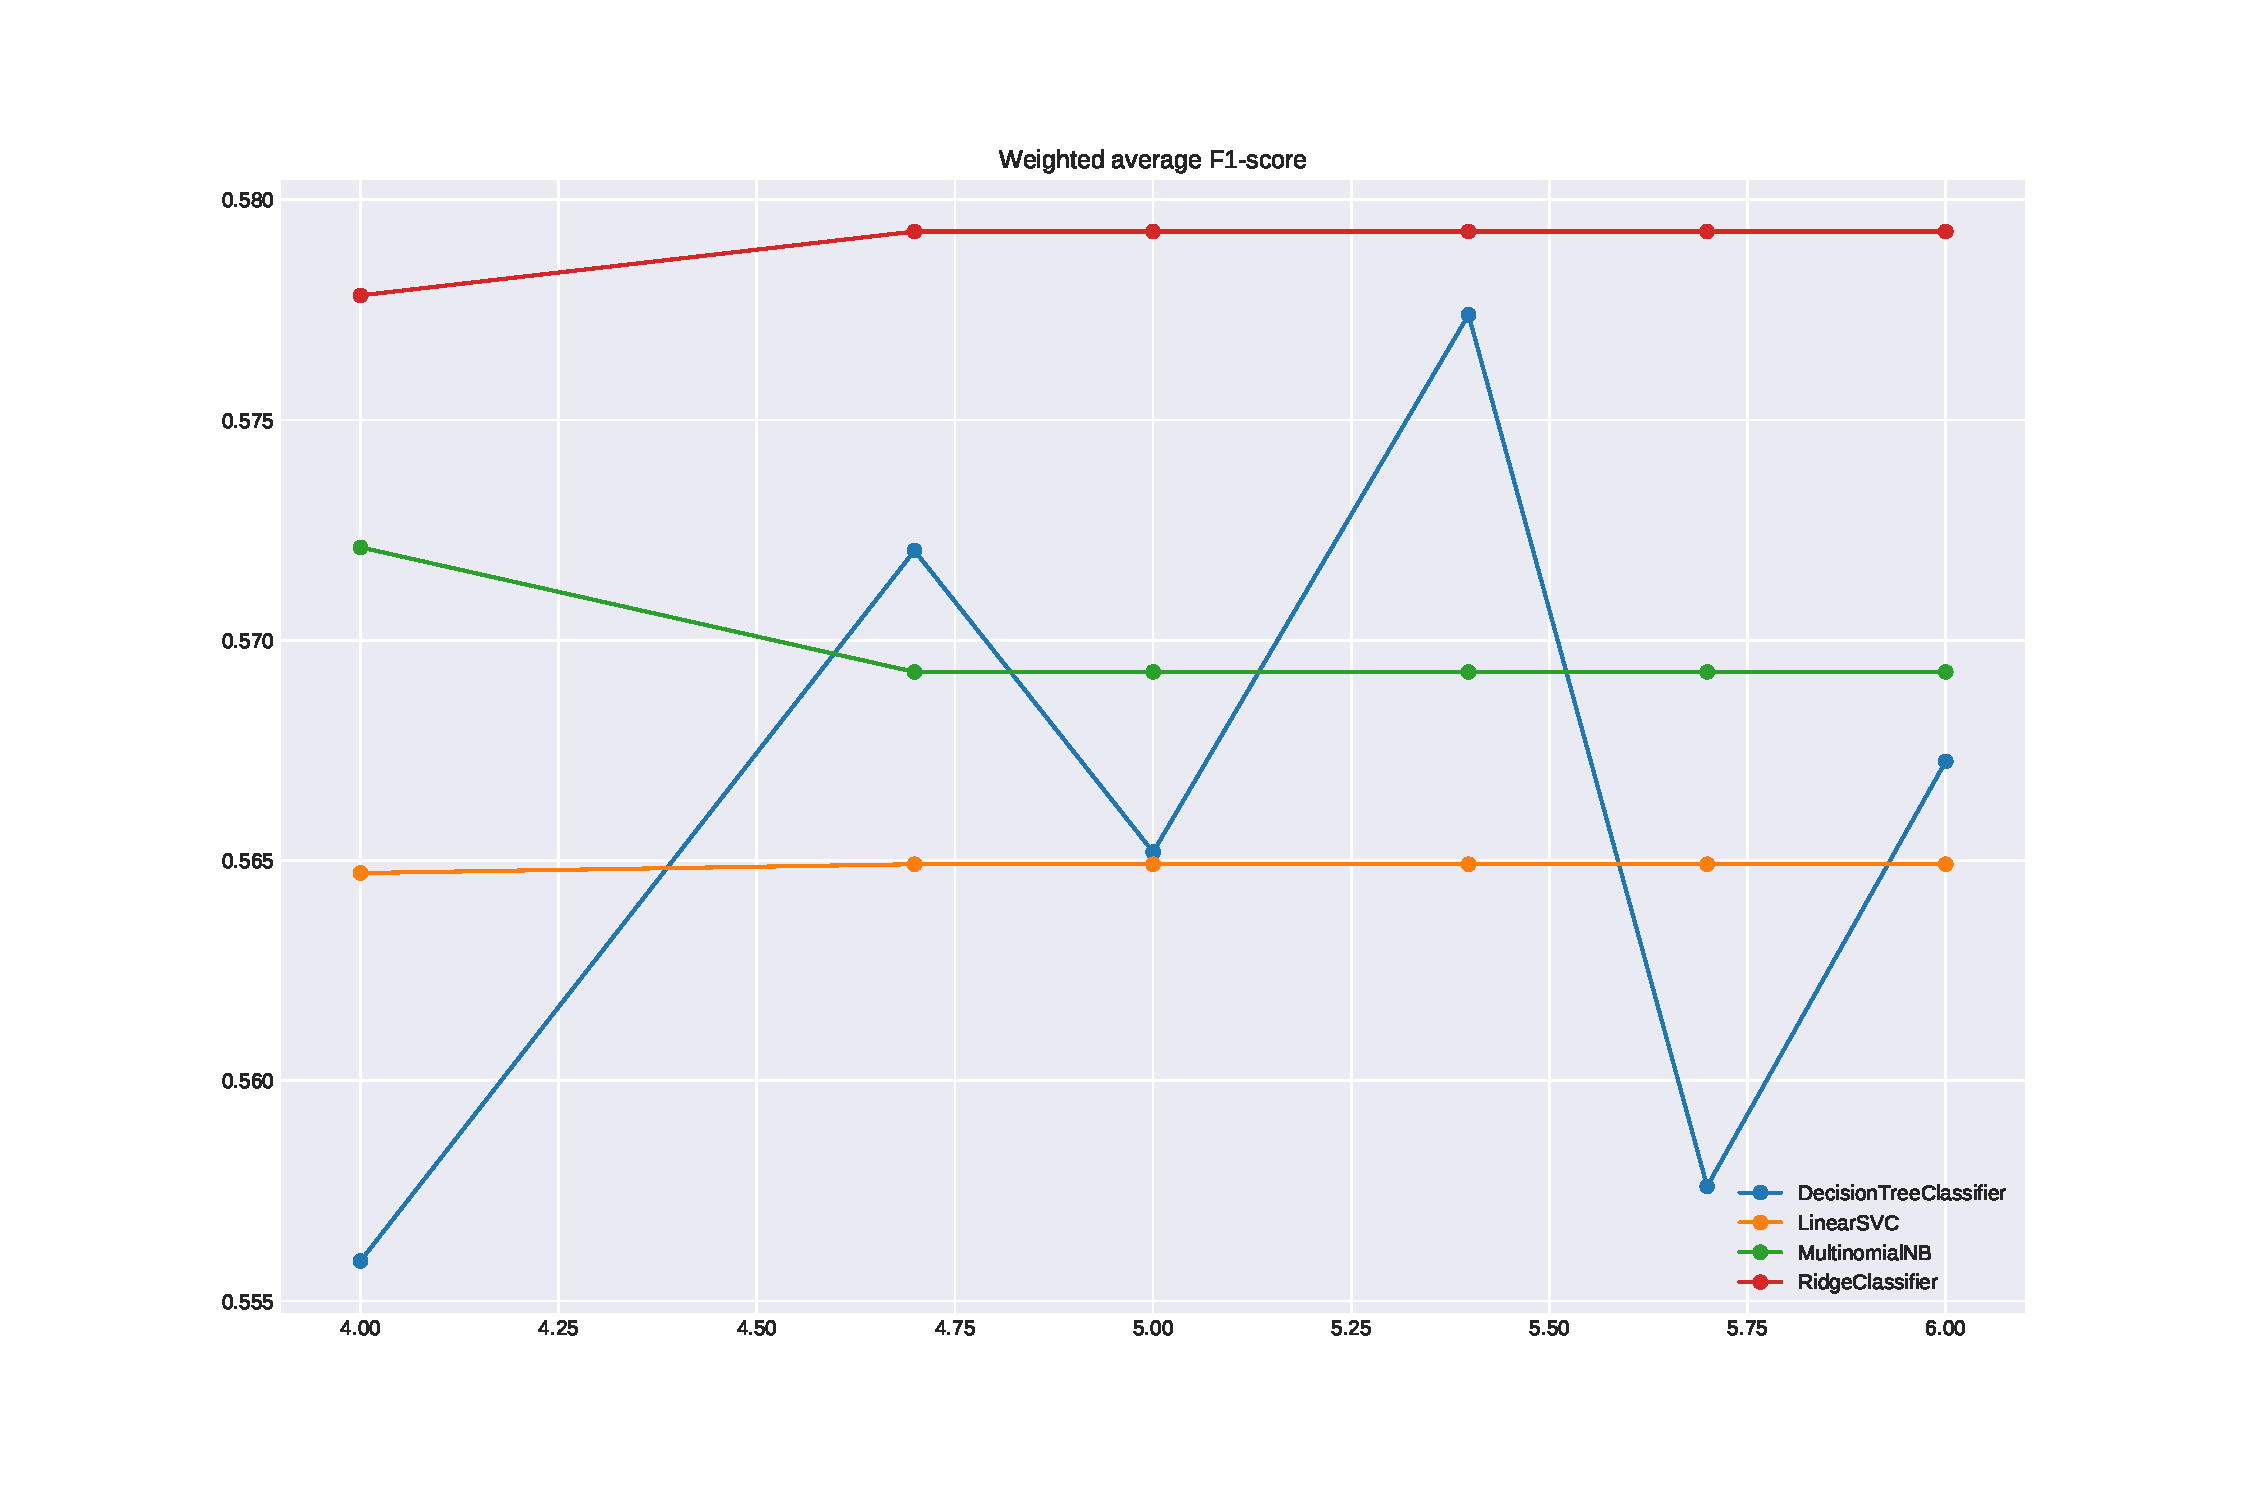
\includegraphics[width=1.2\textwidth]{images/chapitre3/liar-liar_f1_ML}}
 \caption{Weighted average of f1-score, precision and recall of each class. }
 \label{fig:chap3:max_feature3}
\end{figure*}
It goes differently when we focus on a single class. For example, the precision for fake detection is at its maximum for Linear SVM and Ridge Classifier when only 10 features are used. But at the same time, it is at its minium for reliable class. It shows that when trying to optimize the overall model and not only for a single class, it is better to look at the weighted average than at the value for a single class. But it is still important to look at the metrics for a single class because it indicates how it behaves for this class. For instance, in the case of automatic fake news detection, it is important to minimize the number of reliable news misclassified in order to avoid what could be called censorship. 
\begin{figure*}[]
 \centering
 \makebox[\textwidth][c]{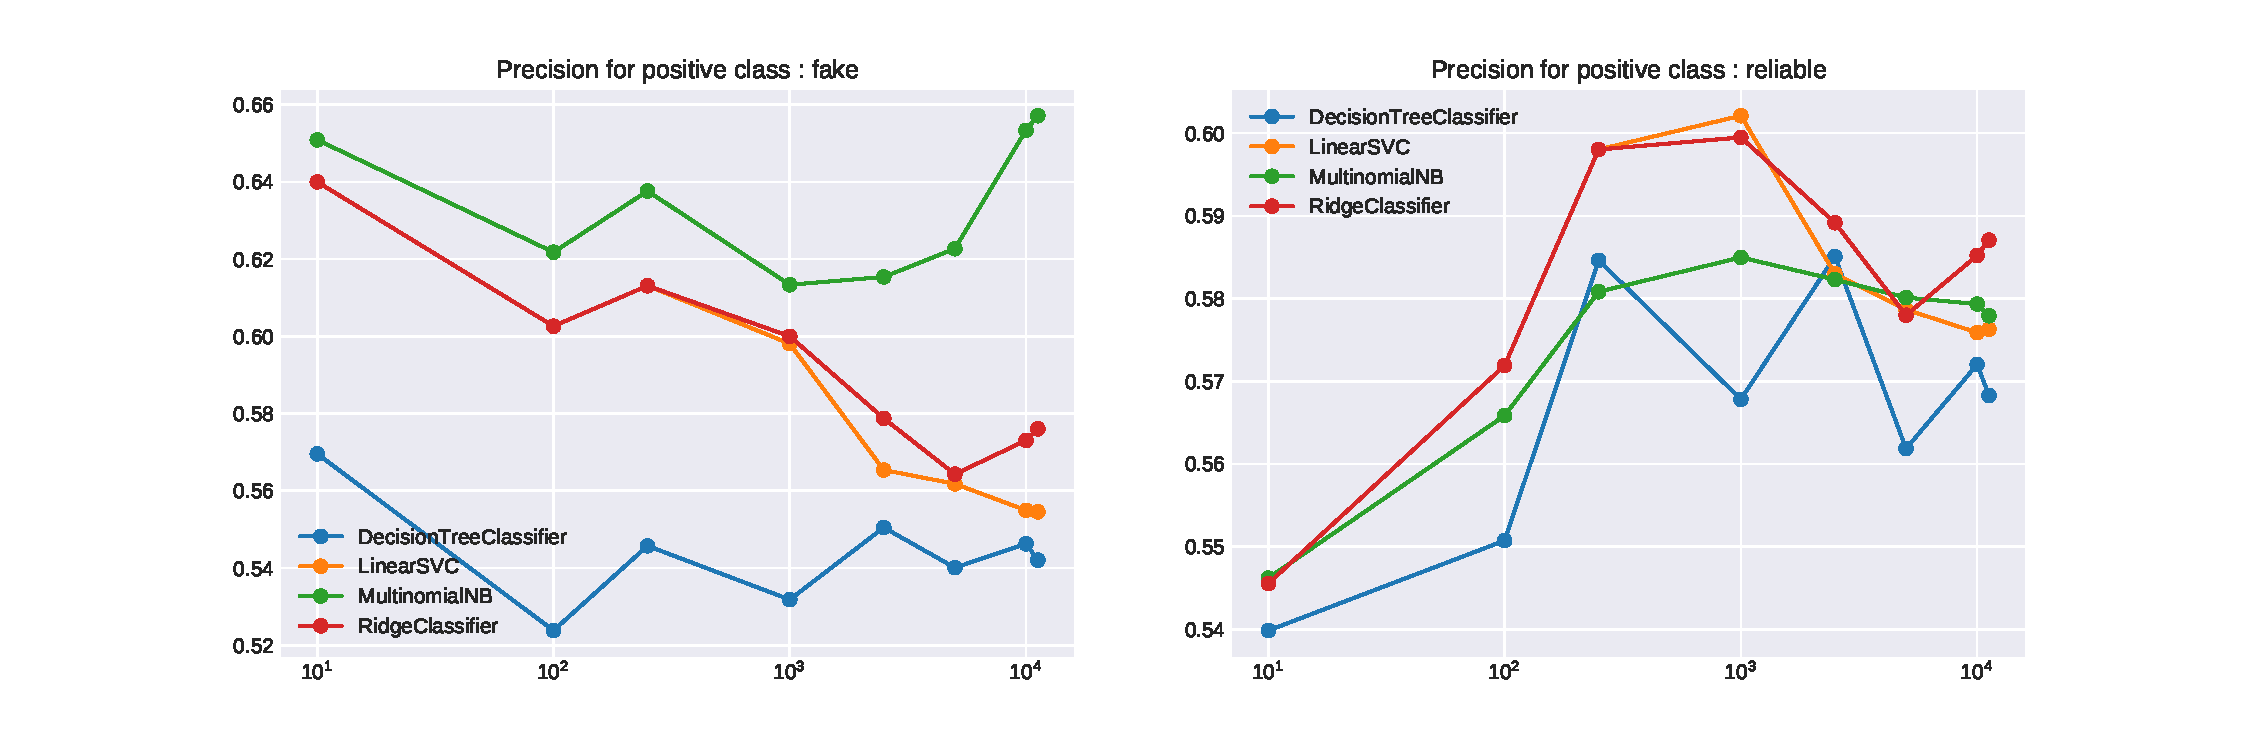
\includegraphics[width=1.2\textwidth]{images/chapitre3/liar-liar_precision_ML}}
 \caption{Precision of the model for each class, the x axes is log scale of the number of features}
 \label{fig:chap3:max_feature1}
\end{figure*}
\begin{figure*}[]
 \centering
 \makebox[\textwidth][c]{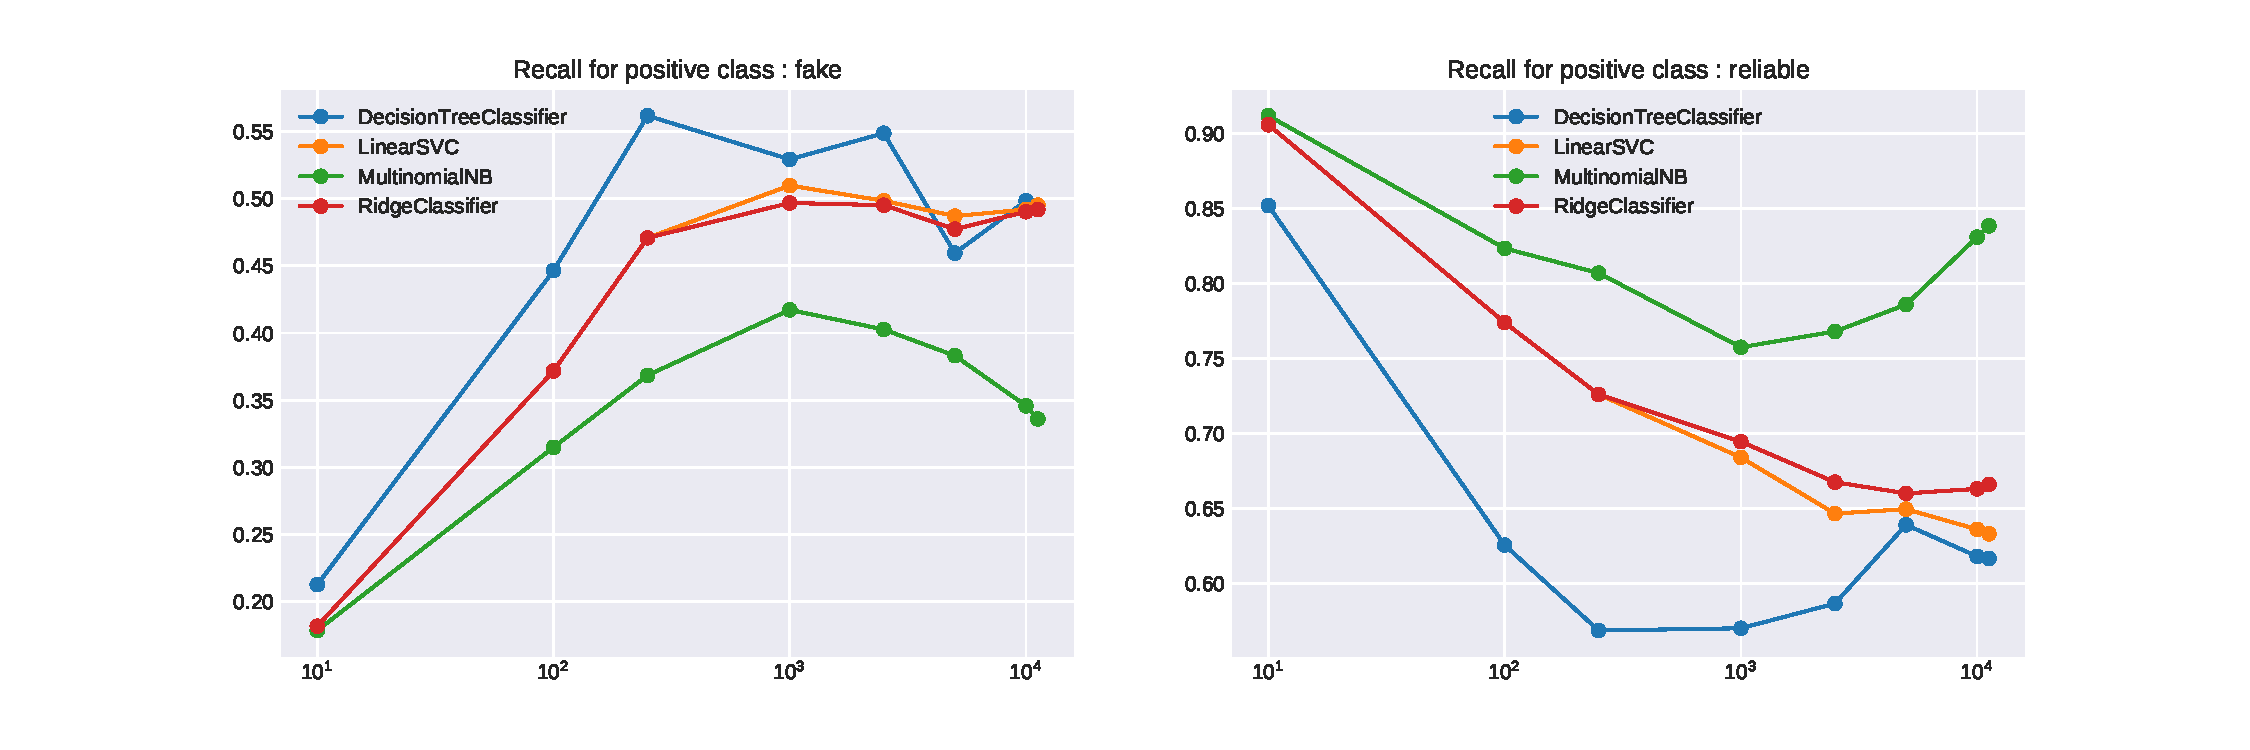
\includegraphics[width=1.2\textwidth]{images/chapitre3/liar-liar_recall_ML}}
 \caption{Precision of the model for each class, the x axes is log scale of the number of features}
 \label{fig:chap3:max_feature2}
\end{figure*}
\section{Models on fake corpus dataset}
\subsection{SMOTE: Synthetic Minority Over-sampling Technique\cite{Chawla2011}}
As it has been shown in \textbf{Chapter \ref{chap2}}, the fake news corpus is unbalanced. Synthetic minority oversampling is a technique that allows generating fake samples from the minor class. It works by randomly choosing one or many nearest neighbours in the minority class. For instance, if the algorithm is set to use 5 nearest neighbours, for each sample it will choose one of its nearest neighbours, and generate a new sample on the segment joining the sample and its neighbour. 
\begin{algorithm}
  \KwData{k = Number of nearest neighbours}
  \KwData{T = number of minority class samples}
  \For{$i \leftarrow 1...T$}{Compute k-nearest neighbours of sample i\;
   Populate(knn, i)\;}
  \caption{SMOTE}
  \label{algo:SMOTE}
\end{algorithm}
\begin{algorithm}
 \KwData{knn = the k-nearest neighbour of sample i}
 \KwData{s = ith sample}
 nn = random\_choice(knn)\;
 newSample = s + rand(0, 1) * (nn - s)\;
 \caption{Populate}
 \label{algo:populate}
\end{algorithm}
\textbf{Algorithm \ref{algo:SMOTE}} and \textbf{\ref{algo:populate}} shows how it works. The first one computes the k-nearest neighbours and the second one computes a new element by randomly choosing one of these neighbours. 
\subsection{Model selection without using SMOTE}
\subsubsection{Hyperparameters tuning}
As for the models trained on the \textbf{liar-liar corpus}, hyper-parameters can be optimized the same way. The average metric for each model with respect to their parameters are shown at \textbf{Figure \ref{fig:chap3:ridge2}, \ref{fig:chap3:dt2}} and \textbf{\ref{fig:chap3:lsvm2}}. \\
\begin{figure*}
 \centering
 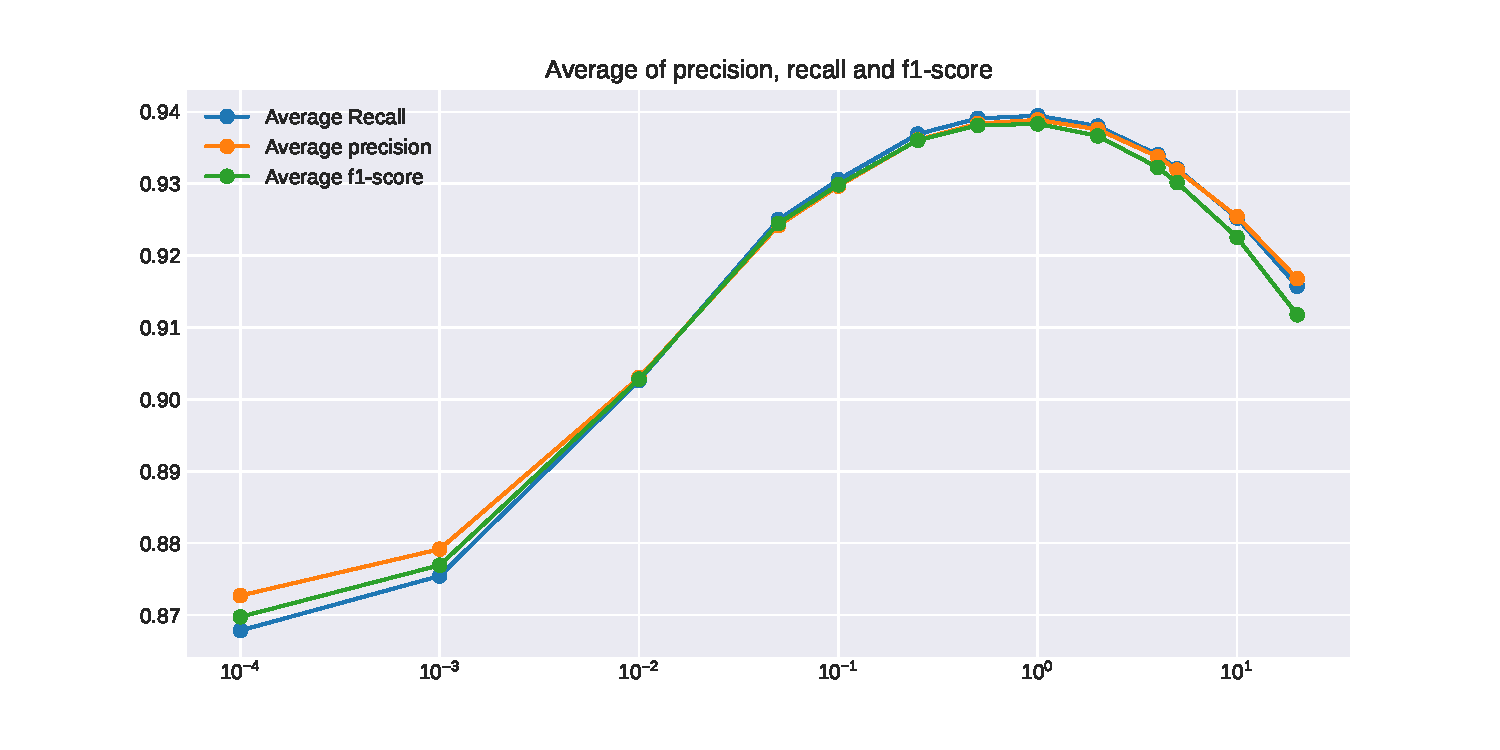
\includegraphics[width=0.8\textwidth]{images/chapitre3/ridge}
 \caption{Metrics value with respect to the penalty parameter for ridge classifier}
 \label{fig:chap3:ridge2}
\end{figure*}
The optimal parameter for the ridge classifier is clearly 1. As well as for the decision tree trained on \textbf{liar-liar} dataset, the optimal maximum depth is of 1000. 
\begin{figure*}
 \centering
 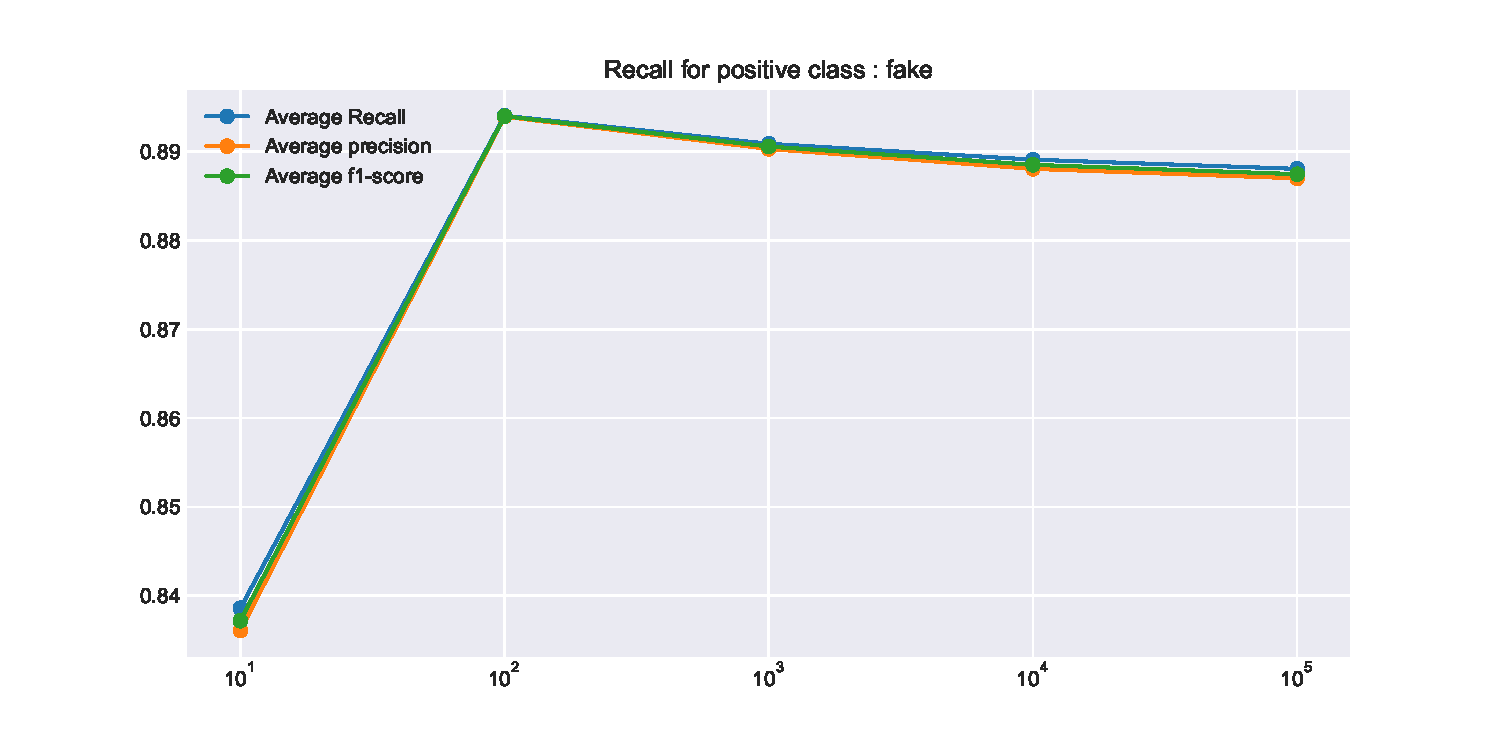
\includegraphics[width=0.8\textwidth]{images/chapitre3/fake-dt}
 \caption{Optimal depth of decision tree.}
 \label{fig:chap3:dt2}
\end{figure*}
And finally, the optimal value for the penalty parameter of the svm is also 1.\\
\begin{figure*}
 \centering
 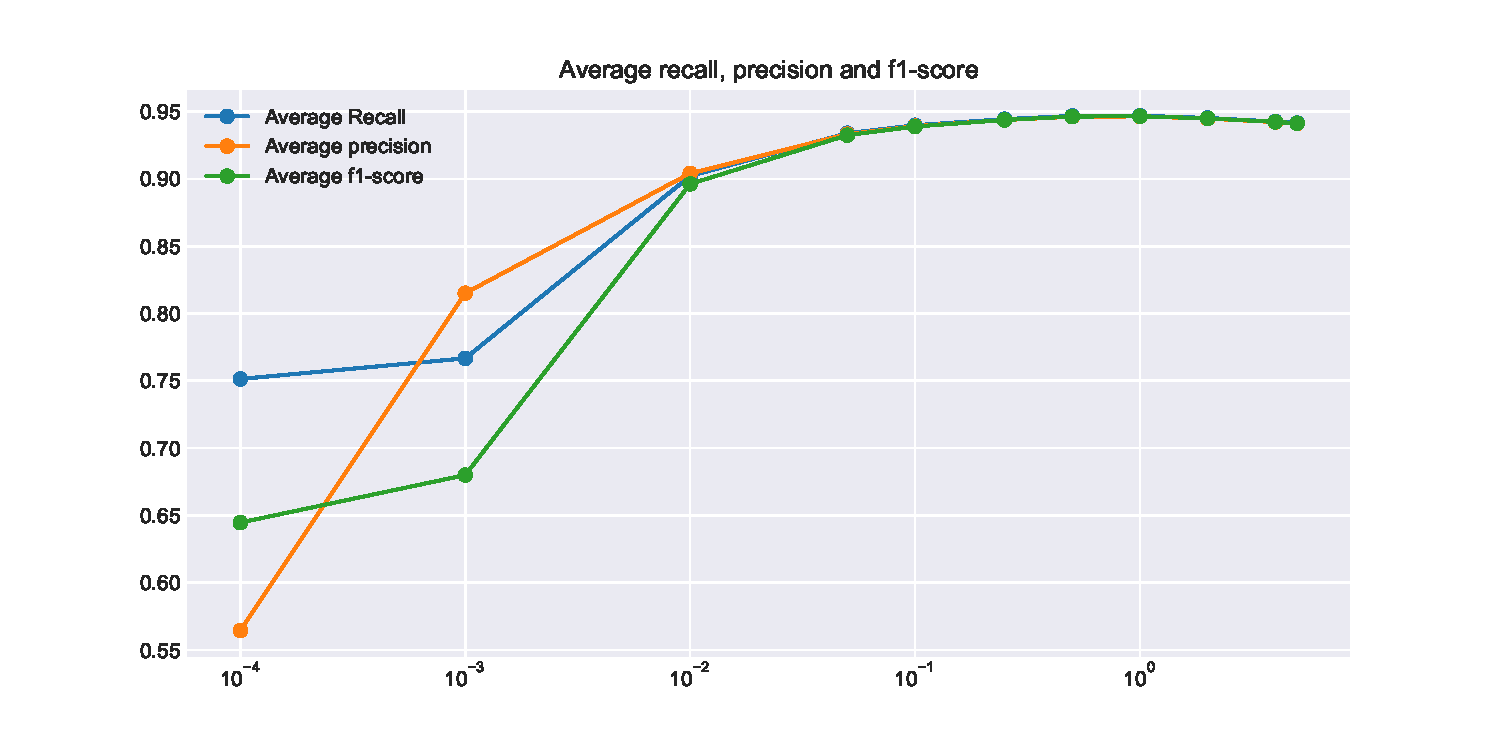
\includegraphics[width=0.8\textwidth]{images/chapitre3/svc_fake}
 \caption{Optimal penalty parameters for linear svm}
 \label{fig:chap3:lsvm2}
\end{figure*}
By looking at \textbf{Figure \ref{fig:chap3:max_feature1}, \ref{fig:chap3:max_feature2}} and \textbf{\ref{fig:chap3:max_feature3}} we can find optimal parameters for the number of features used in TF-IDF. It shows that linear svm and ridge classifiers are the ones that perform the best, having an average precision of sligtly more than $94\%$ for the linear svm and $94\%$ for the ridge classifier. They achieve these performances from $50,000$ features and does not decrease. On the other hand, Na\"{i}ve-Bayes reaches a pike at $100,000$ features and greatly decrease afterward. \\
\begin{figure*}
 \centering
 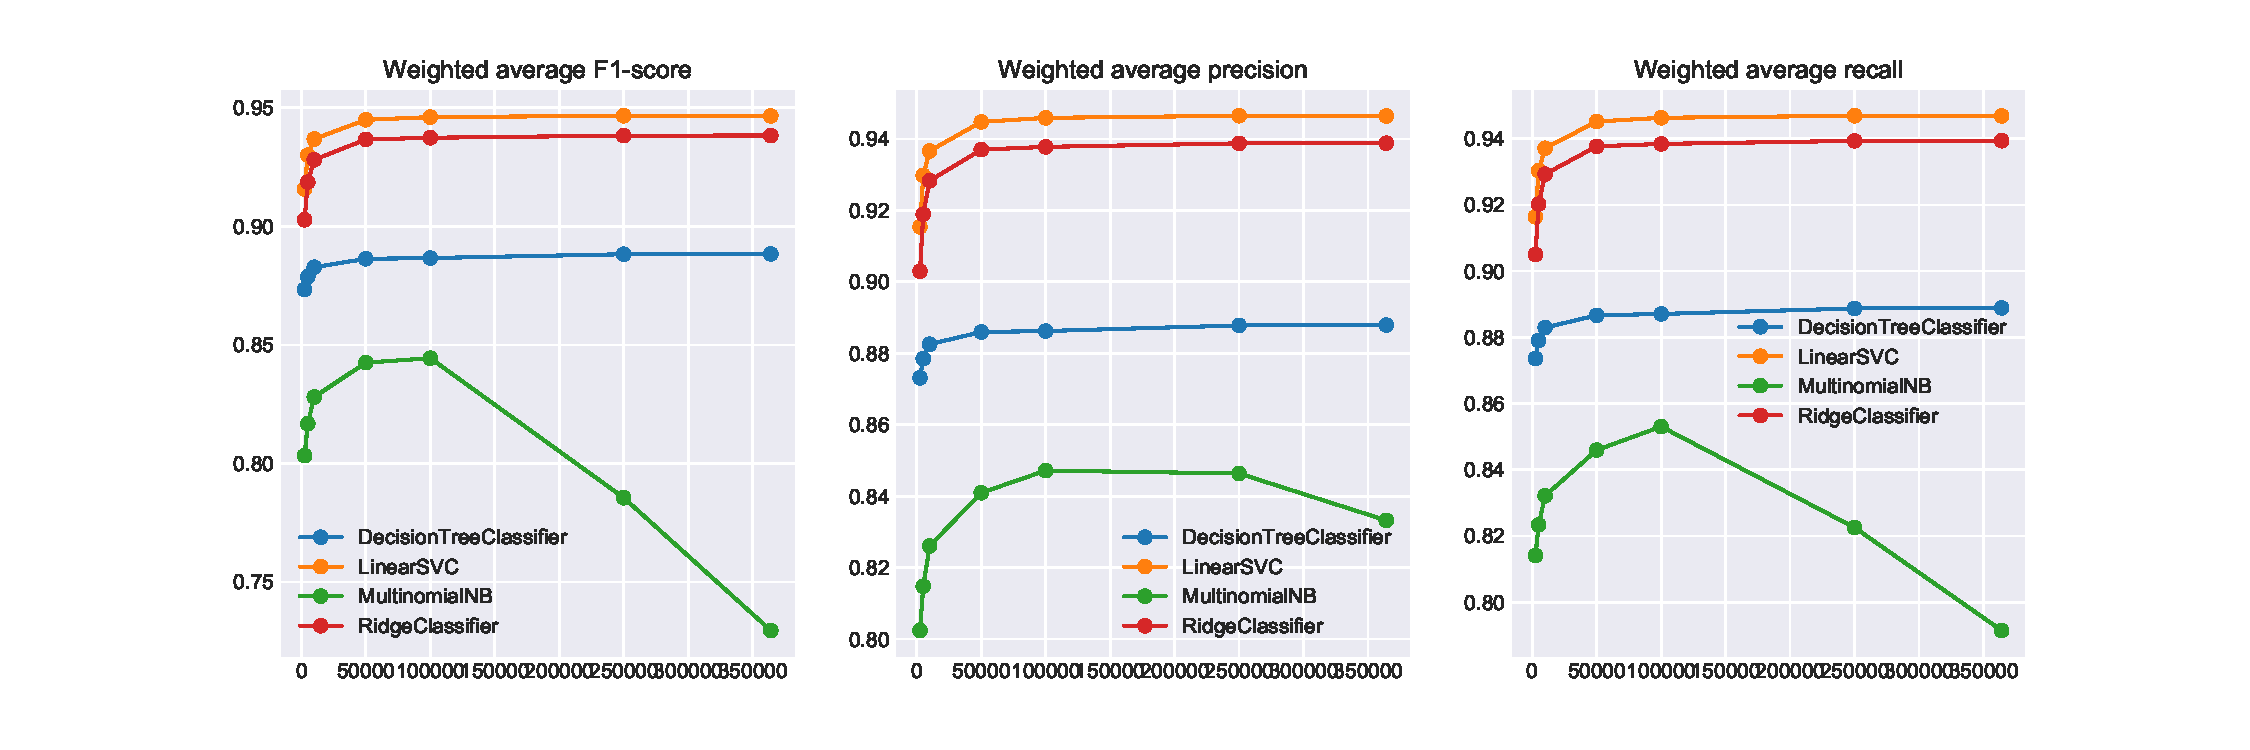
\includegraphics[width=0.8\textwidth]{images/chapitre3/ML_fake_average}
 \caption{Average recall, precision and f1-score wti respect to the maximum number of features.}
 \label{fig:chap3:max_feat1}
\end{figure*}
\begin{figure*}
 \centering
 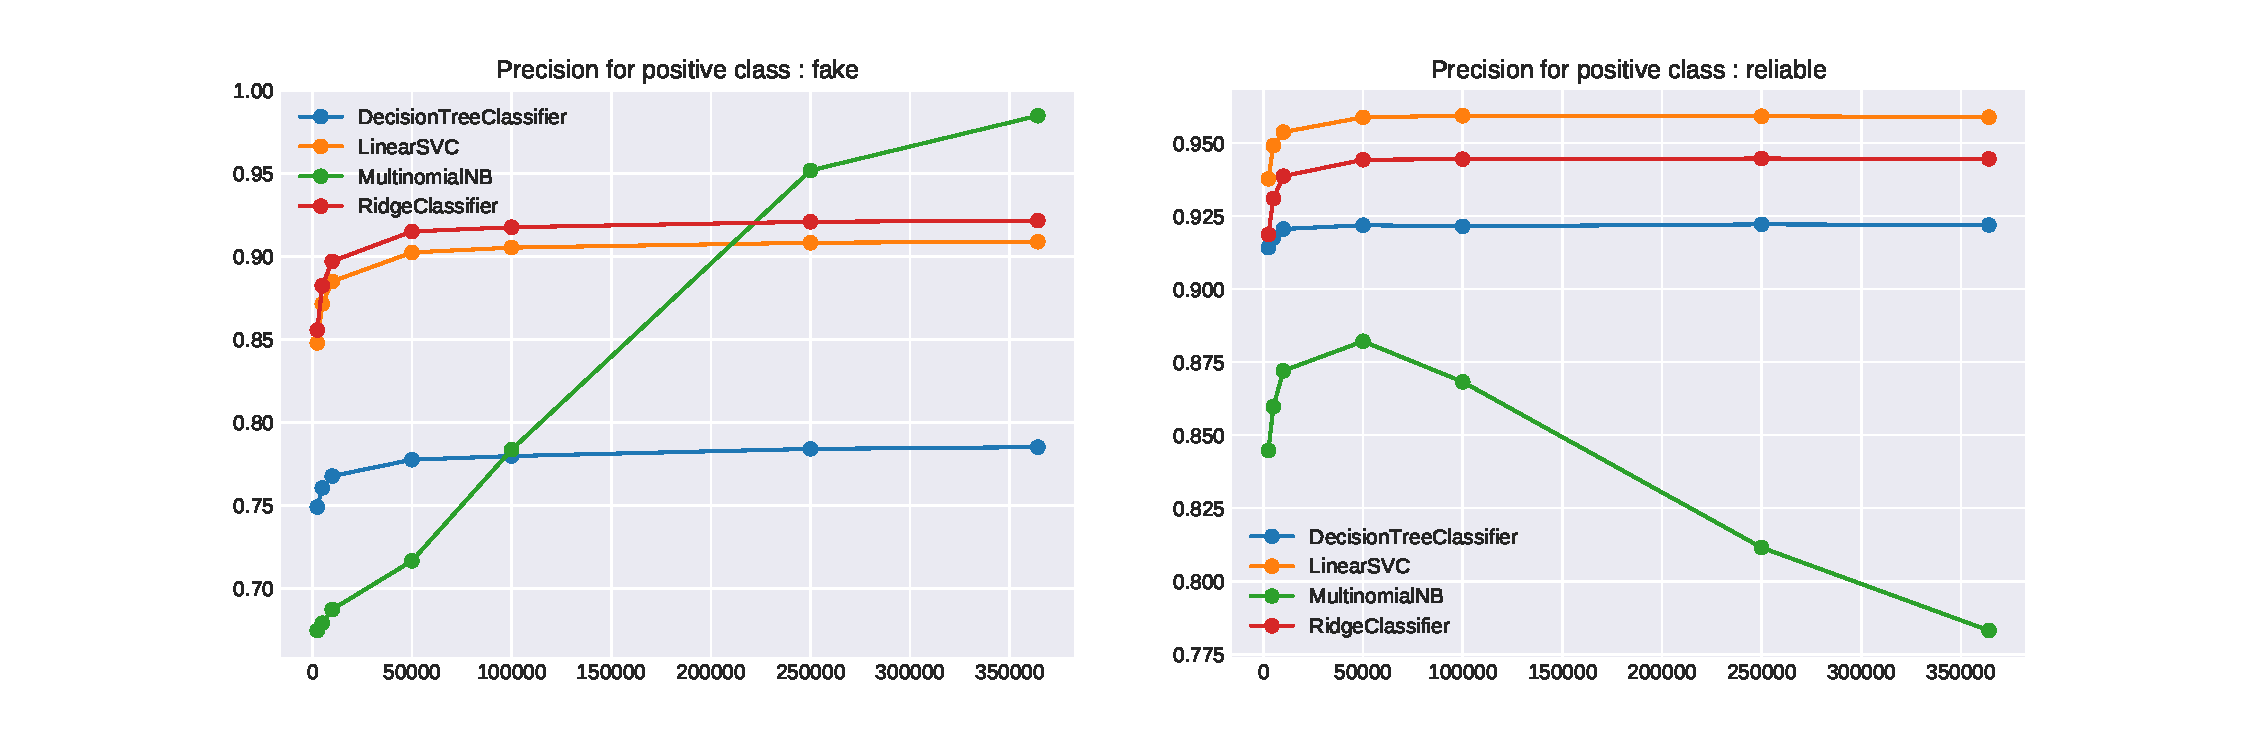
\includegraphics[width=0.8\textwidth]{images/chapitre3/ML_fake_precision}
 \caption{Precision for fake and reliable class for each model with respect to the maximum number of features}
 \label{fig:chap3:max_feat2}
\end{figure*}
\begin{figure*}
 \centering
 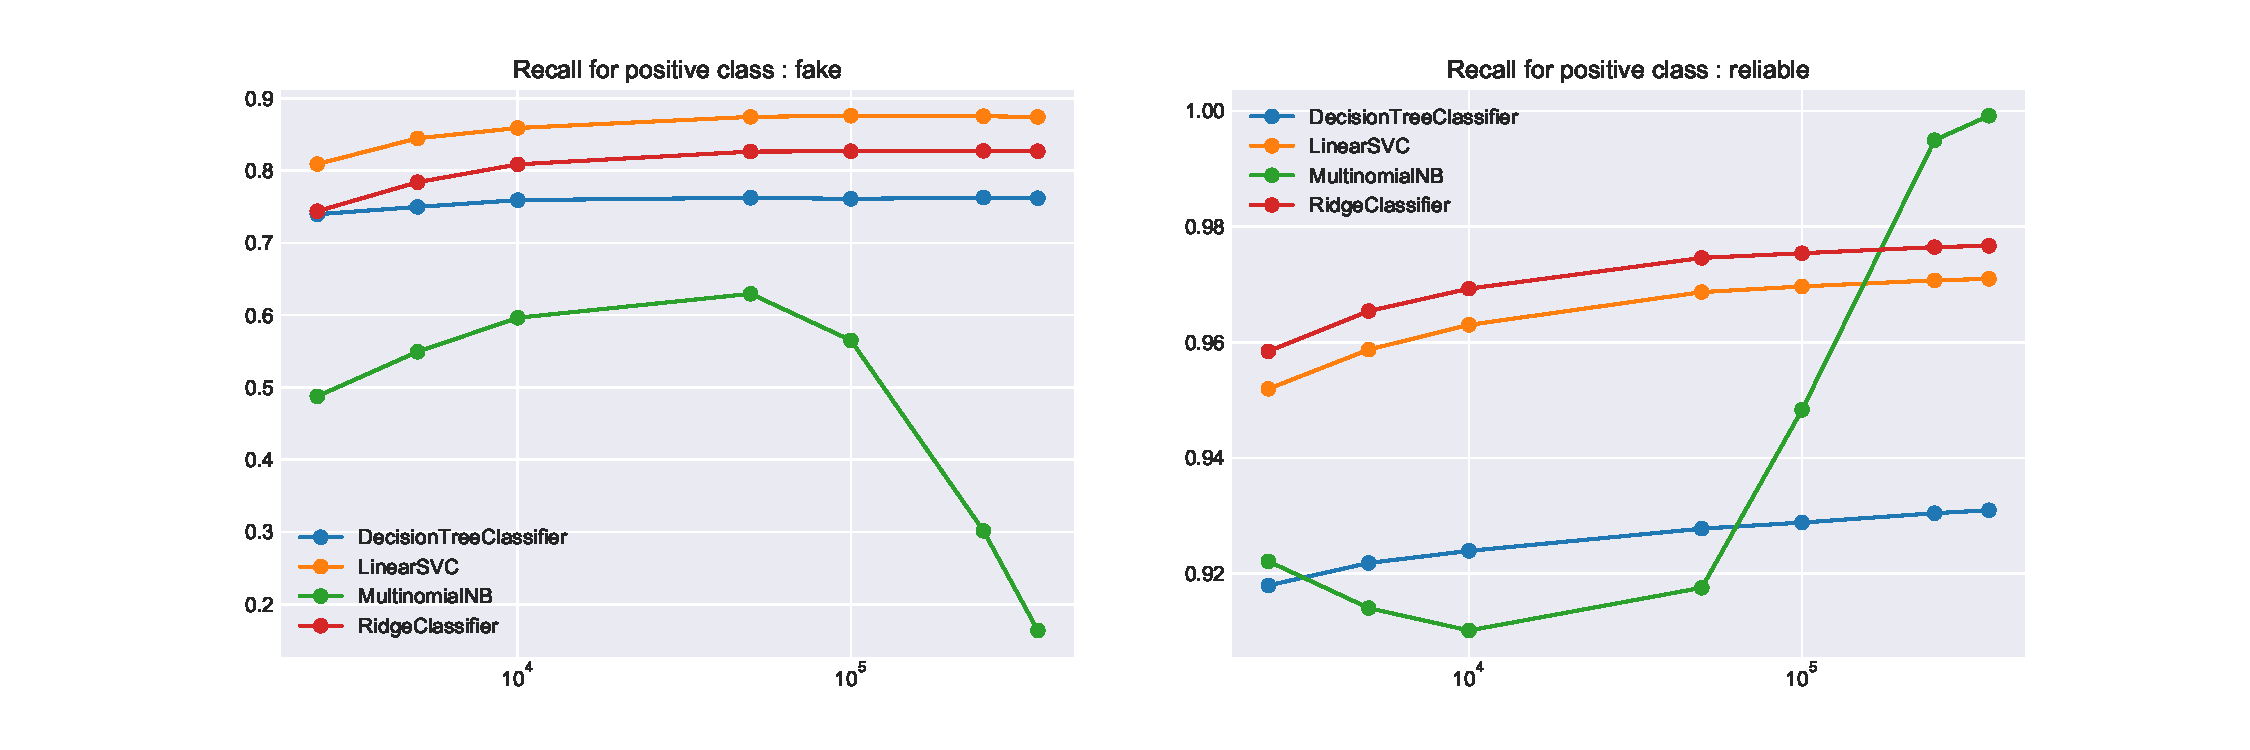
\includegraphics[width=0.8\textwidth]{images/chapitre3/ML_fake_recall}
 \caption{Recall for fake and reliable class for each model with respect to the maximum number of features}
 \label{fig:chap3:max_feat3}
\end{figure*}

\textbf{Figure \ref{fig:chap3:max_feature3}} shows why it is important to look at all the metrics, because Na\"{i}ve-Bayes reaches a recall of 1 for the reliable class and close to 0 for the fake class, which means that almost all texts are classified as reliable. This can be verified by looking at \textbf{Figure \ref{fig:chap3:confMat1}}, only a small proportion of true fake is actually classified as it.
\begin{figure*}
 \centering
 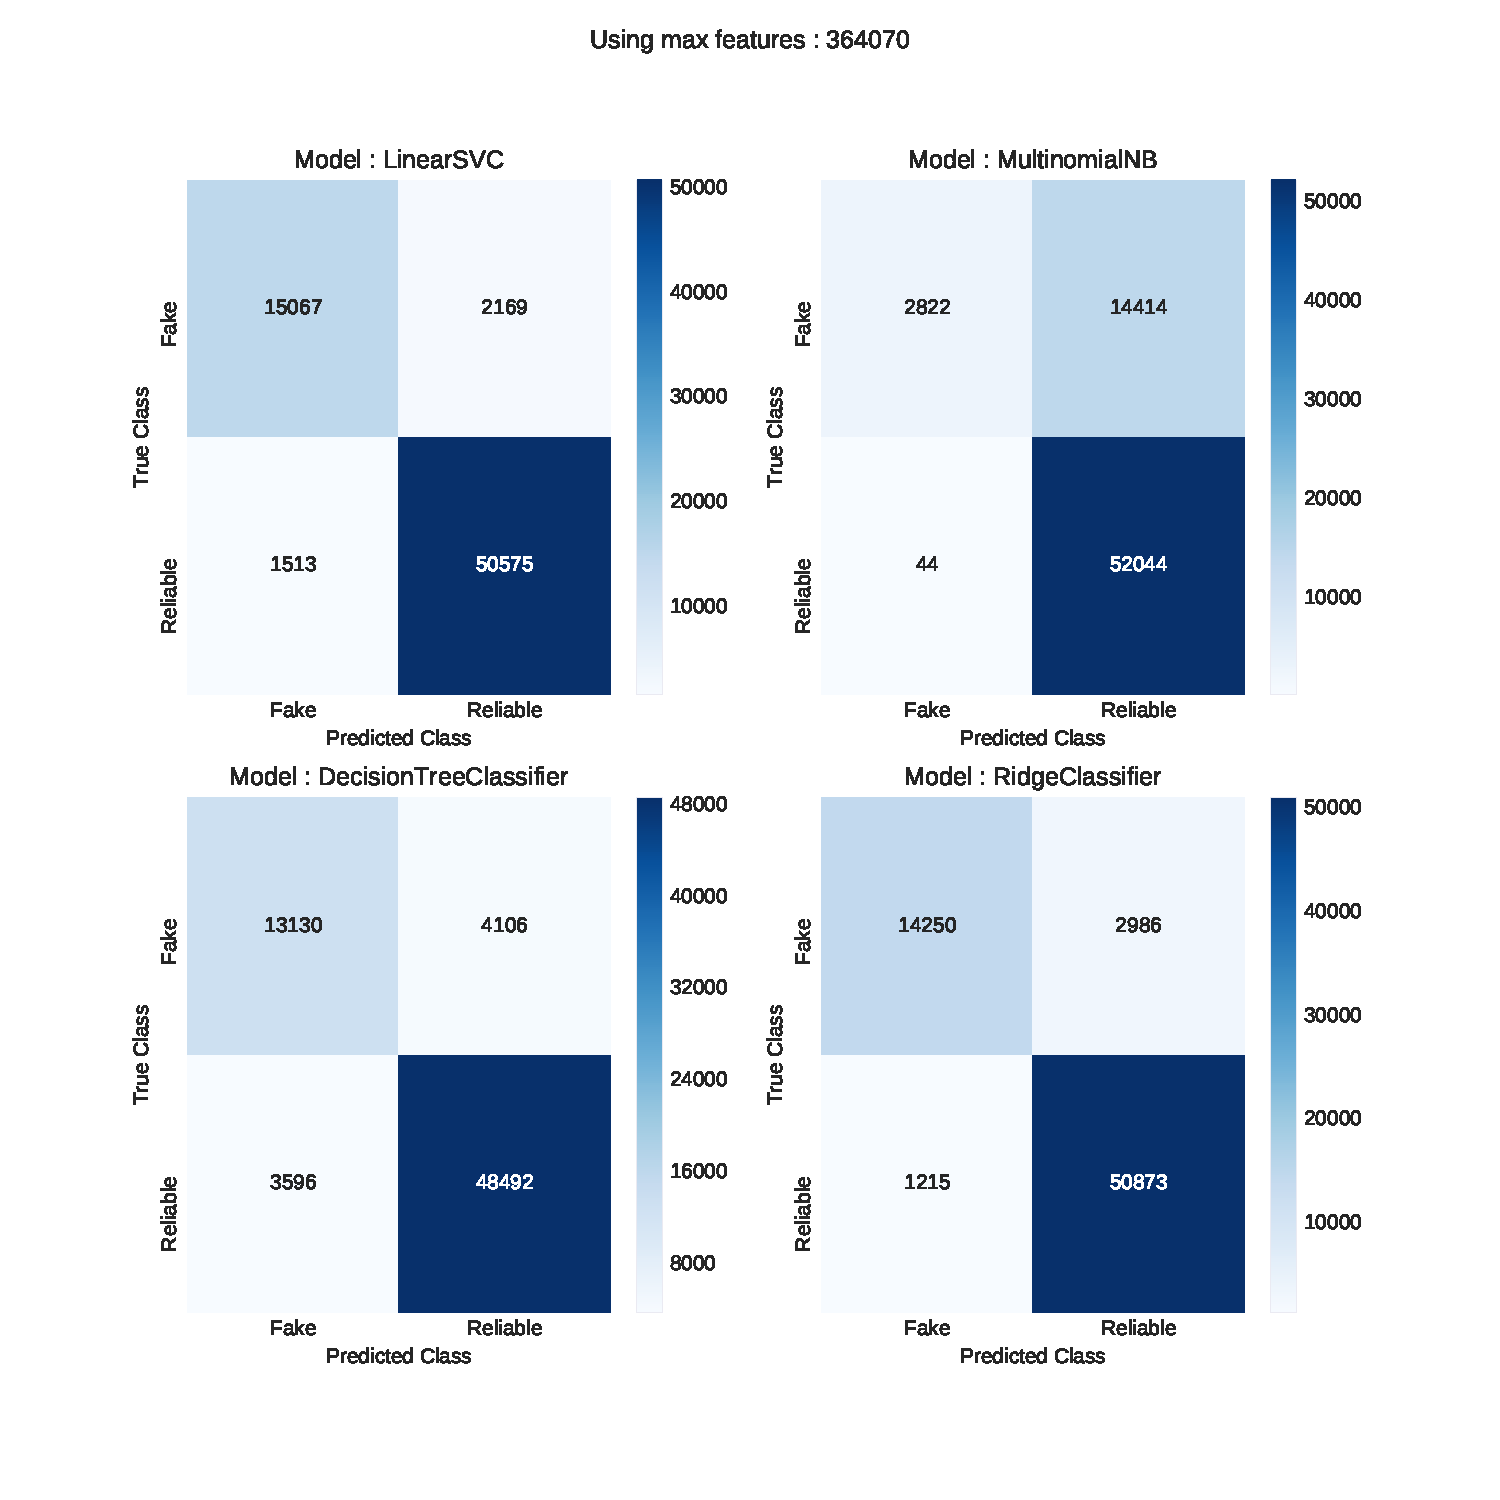
\includegraphics[width=0.5\textwidth]{images/chapitre3/confMat_fake_364070}
 \caption{Confusion matrix for each model using $364,070$ features}
 \label{fig:chap3:confMat1}
\end{figure*}
\subsection{Model selection with SMOTE}
The first thing that can be noticed at \textbf{Figure \ref{fig:chap3:ridge3}, \ref{fig:chap3:dt3}, \ref{fig:chap3:lsvm3}, \ref{fig:chap3:smote_max_feat1}, \ref{fig:chap3:smote_max_feat2}} and \textbf{\ref{fig:chap3:smote_max_feat3}} is that the two models that worked the best without applying SMOTE method, linear SVM and ridge classifiers are still the ones that perform the best. By comparing \textbf{Figure \ref{fig:chap3:lsvm2}} and \textbf{Figure \ref{fig:chap3:lsvm3}} we can see that it works better when applying a smaller regularization parameter. It goes from $0.66\%$ of accuracy to  $0.86\%$ of accuracy thus acting as a regularization. The same does not apply to ridge classifiers. \\
\begin{figure*}
 \centering
 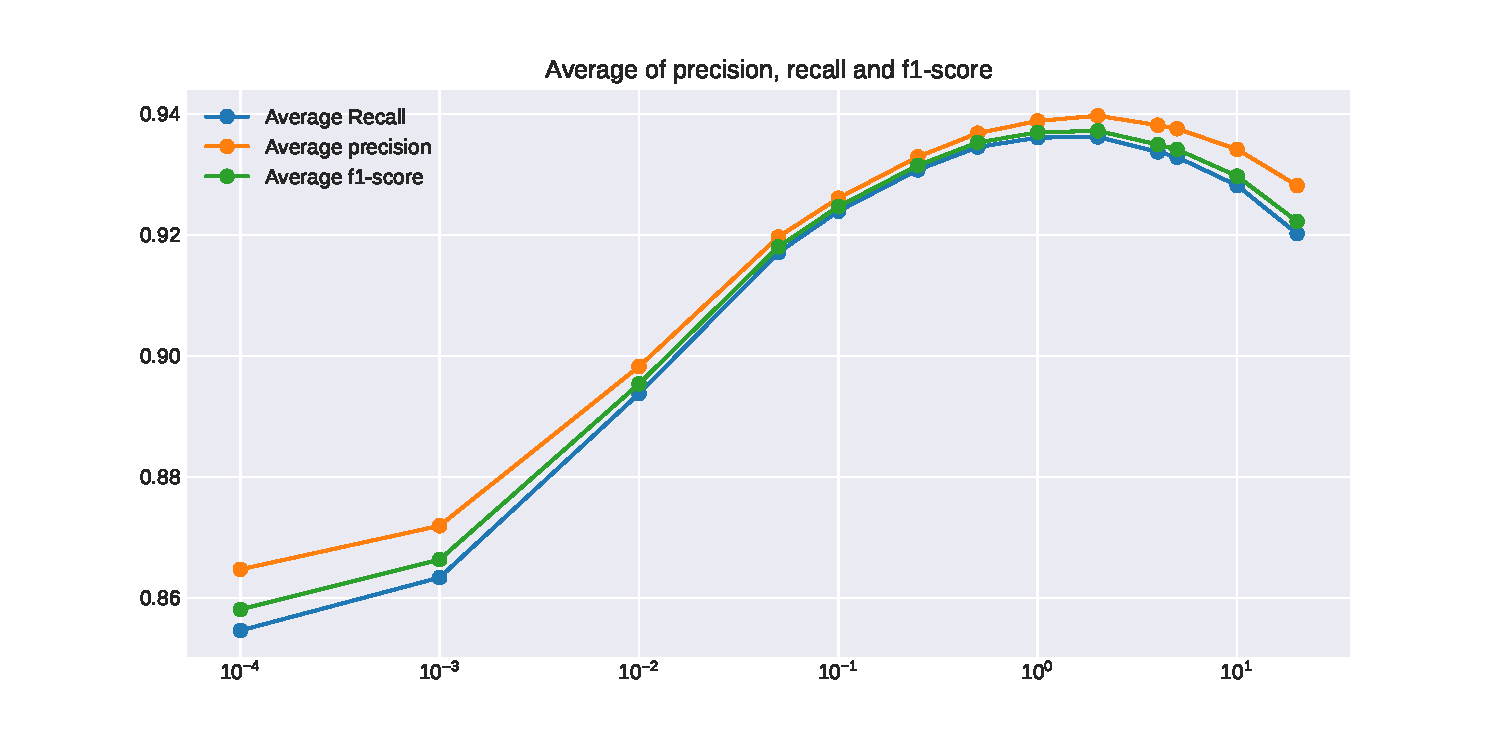
\includegraphics[width=0.8\textwidth]{images/chapitre3/ridge+smote}
 \caption{Metrics value with respect to the penalty parameter for ridge classifiers when using SMOTE.}
 \label{fig:chap3:ridge3}
\end{figure*}
It also has a huge impact on how Na\"{i}ve-Bayes behaves as it removes overfitting when using a larger number of features in TF-IDF, leading to a few percent of accuracy increase. \\
\begin{figure*}
 \centering
 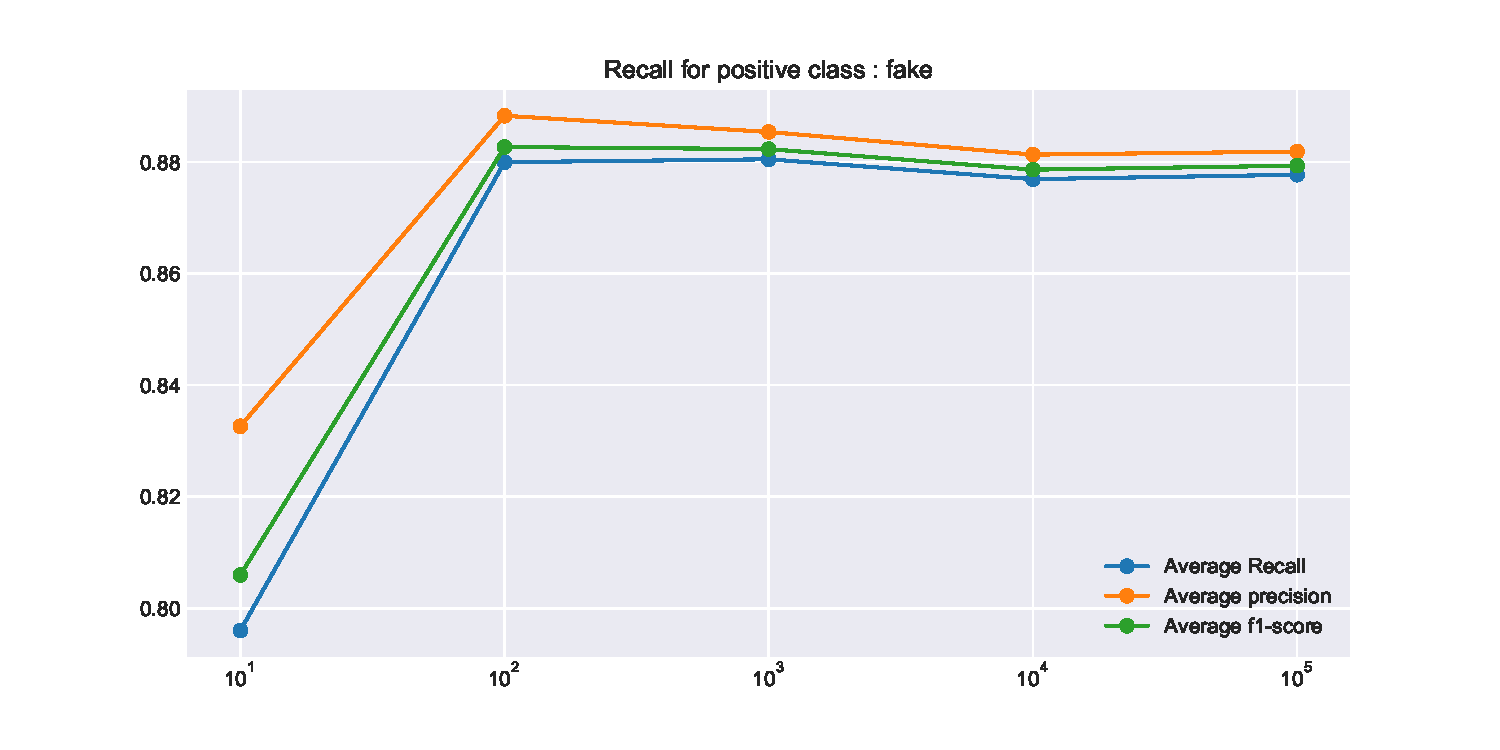
\includegraphics[width=0.8\textwidth]{images/chapitre3/fake-dt-SMOTE}
 \caption{Optimal depth of decision tree when using SMOTE.}
 \label{fig:chap3:dt3}
\end{figure*}
\begin{figure*}
 \centering
 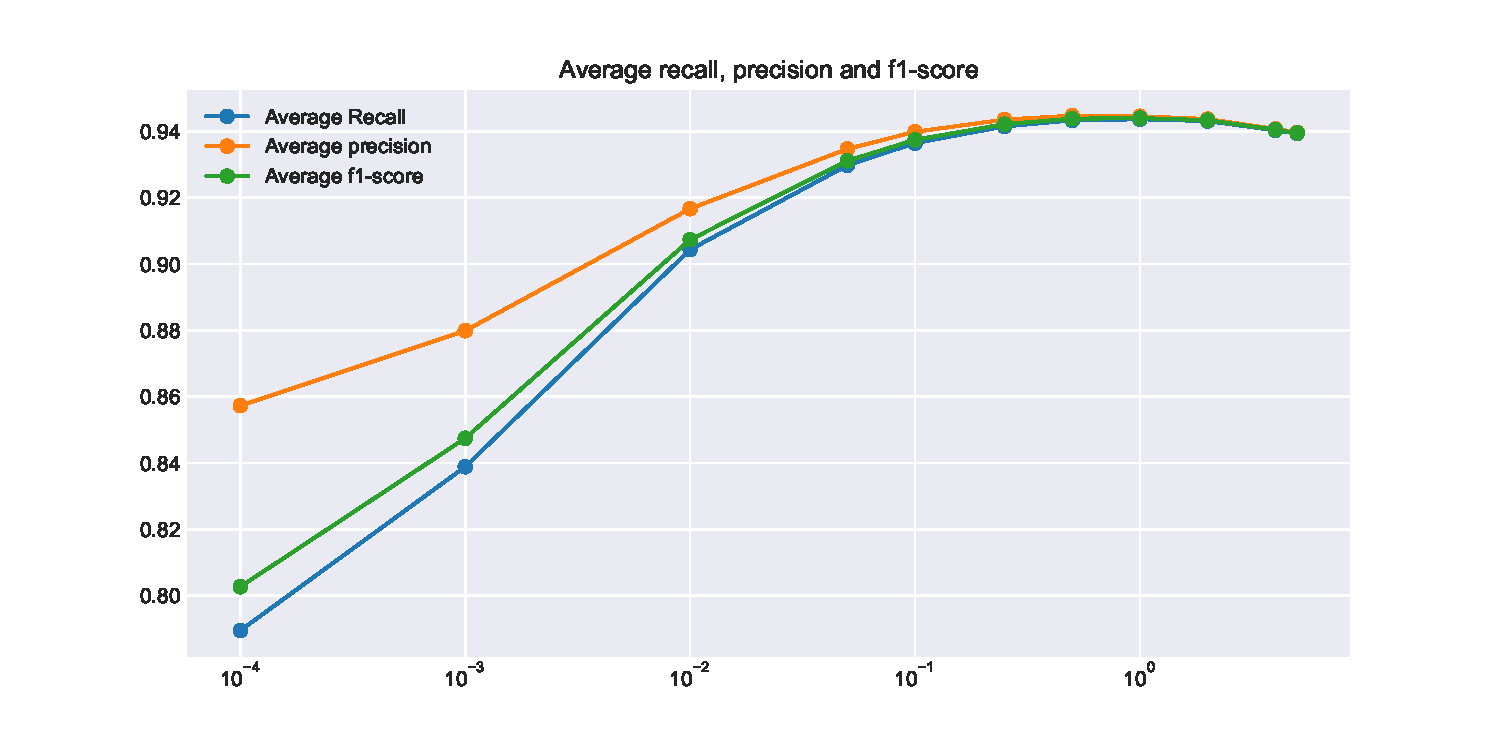
\includegraphics[width=0.8\textwidth]{images/chapitre3/svc_fake_smote}
 \caption{Optimal penalty parameters for linear svm when using SMOTE}
 \label{fig:chap3:lsvm3}
\end{figure*}

\begin{figure*}
 \centering
 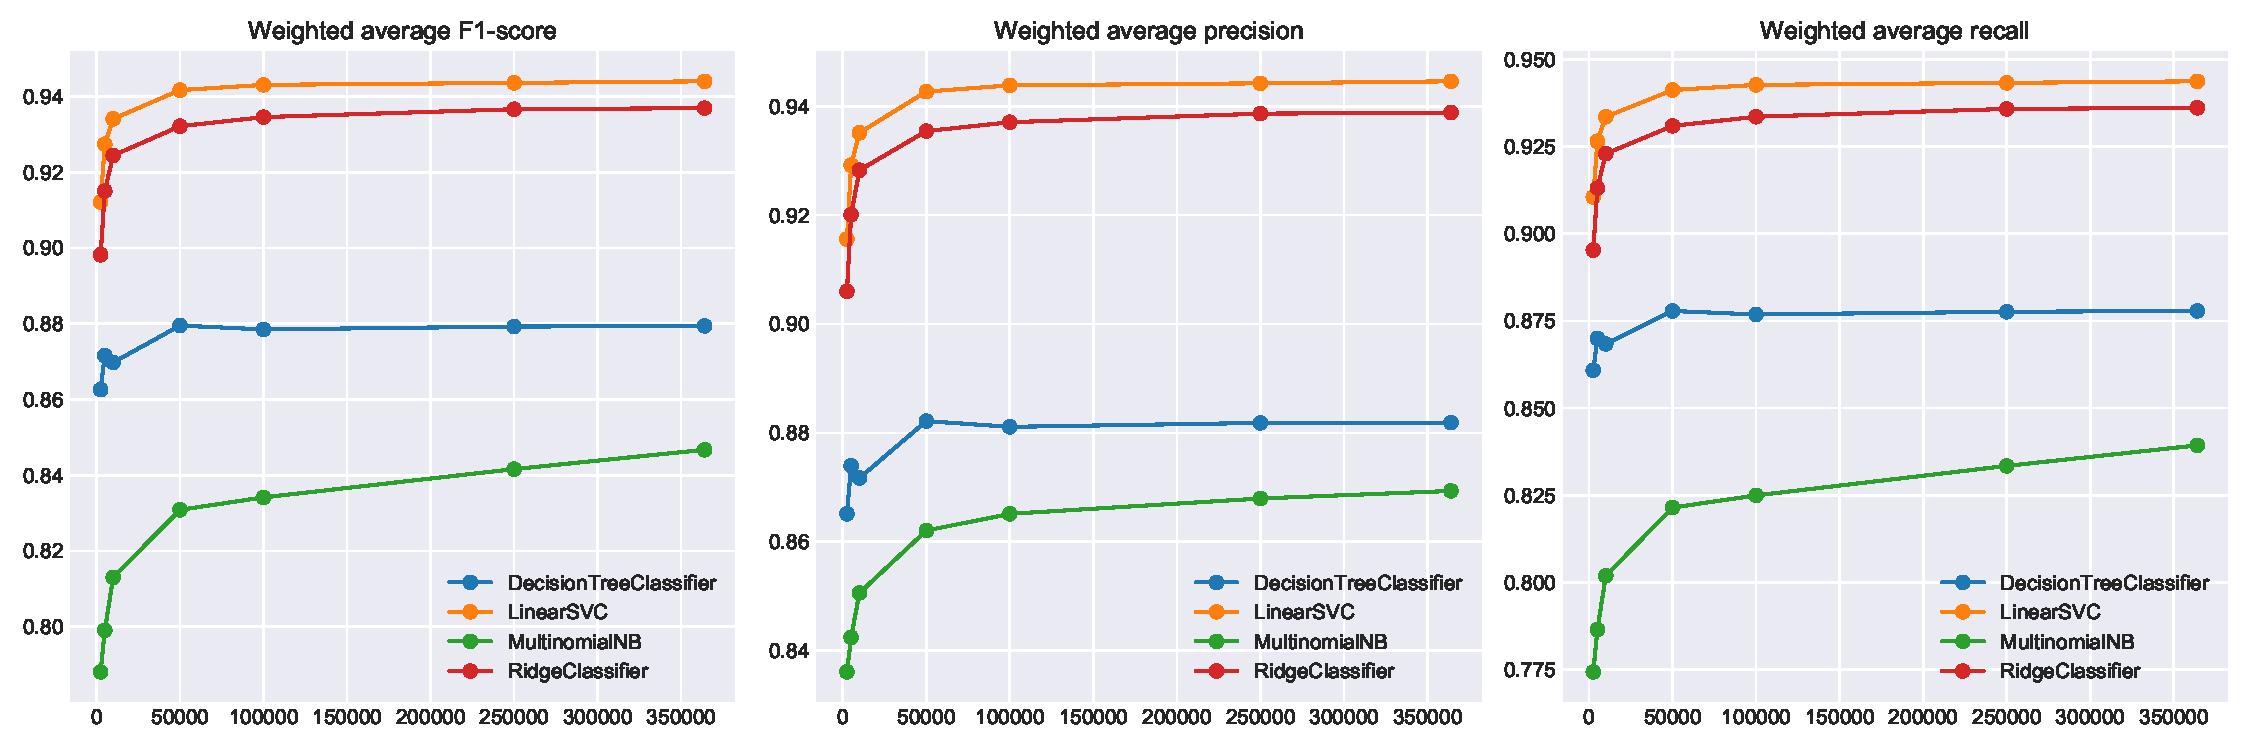
\includegraphics[width=0.8\textwidth]{images/chapitre3/ML_SMOTE_fake_average}
 \caption{Average recall, precision and f1-score wti respect to the maximum number of features.}
 \label{fig:chap3:smote_max_feat1}
\end{figure*}
\begin{figure*}
 \centering
 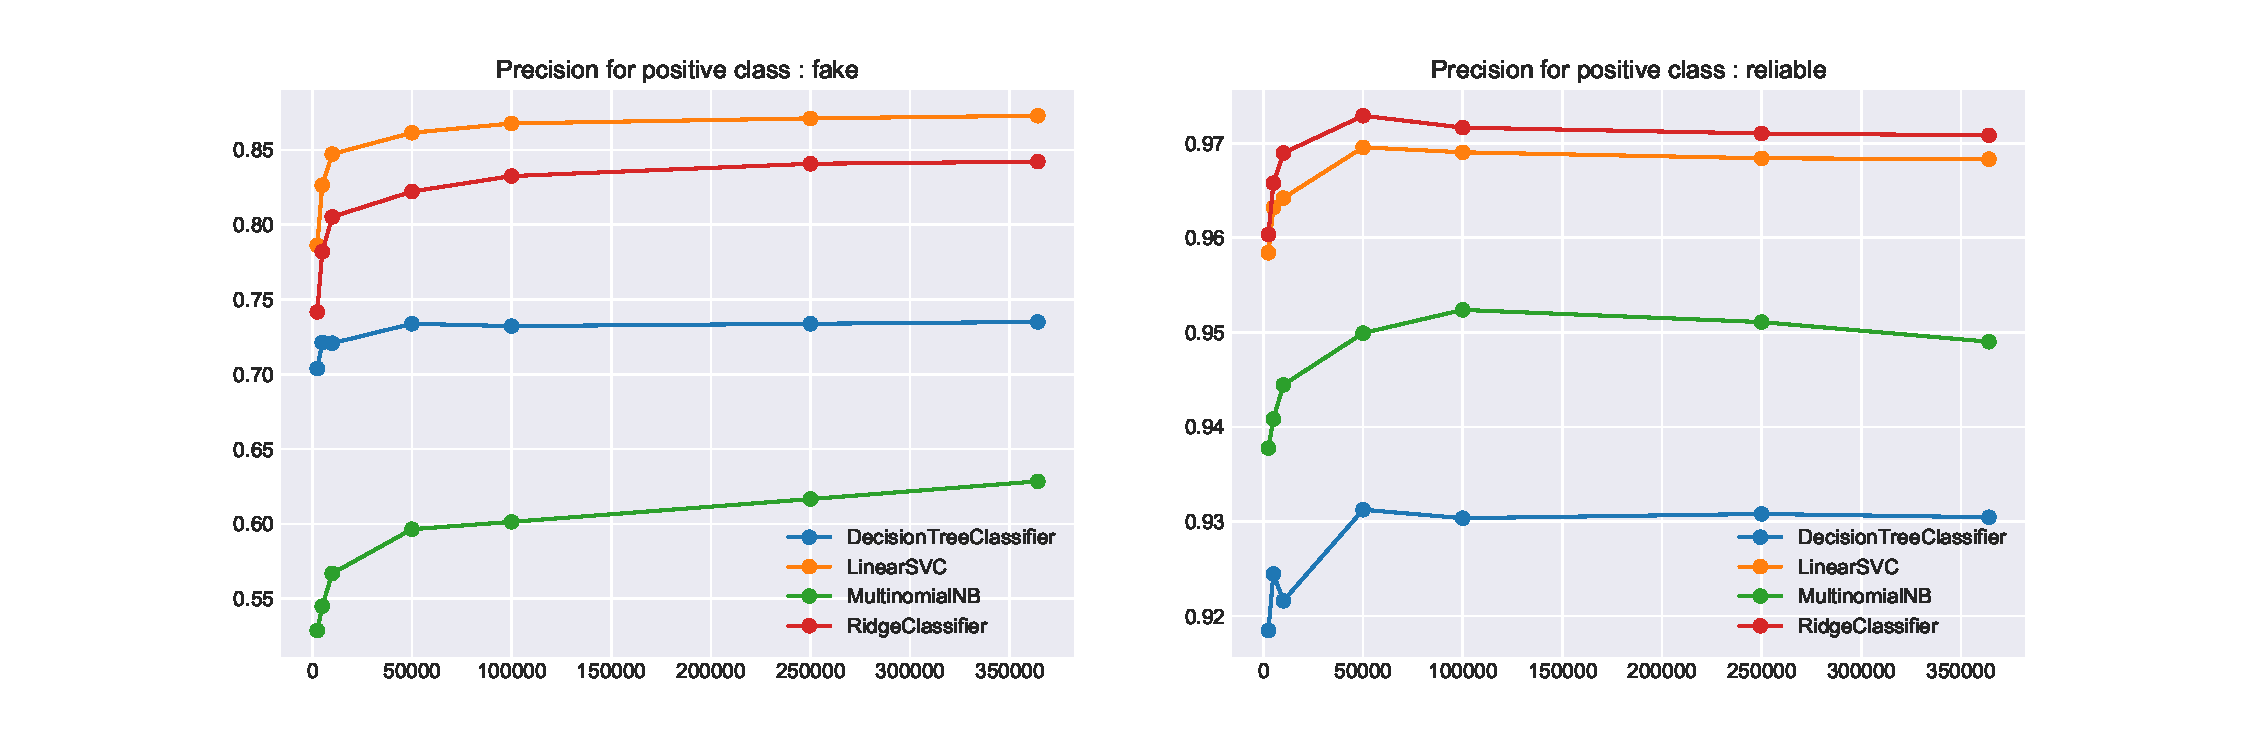
\includegraphics[width=0.8\textwidth]{images/chapitre3/ML_SMOTE_fake_precision}
 \caption{Precision for fake and reliable class for each model with respect to the maximum number of features}
 \label{fig:chap3:smote_max_feat2}
\end{figure*}
\begin{figure*}
 \centering
 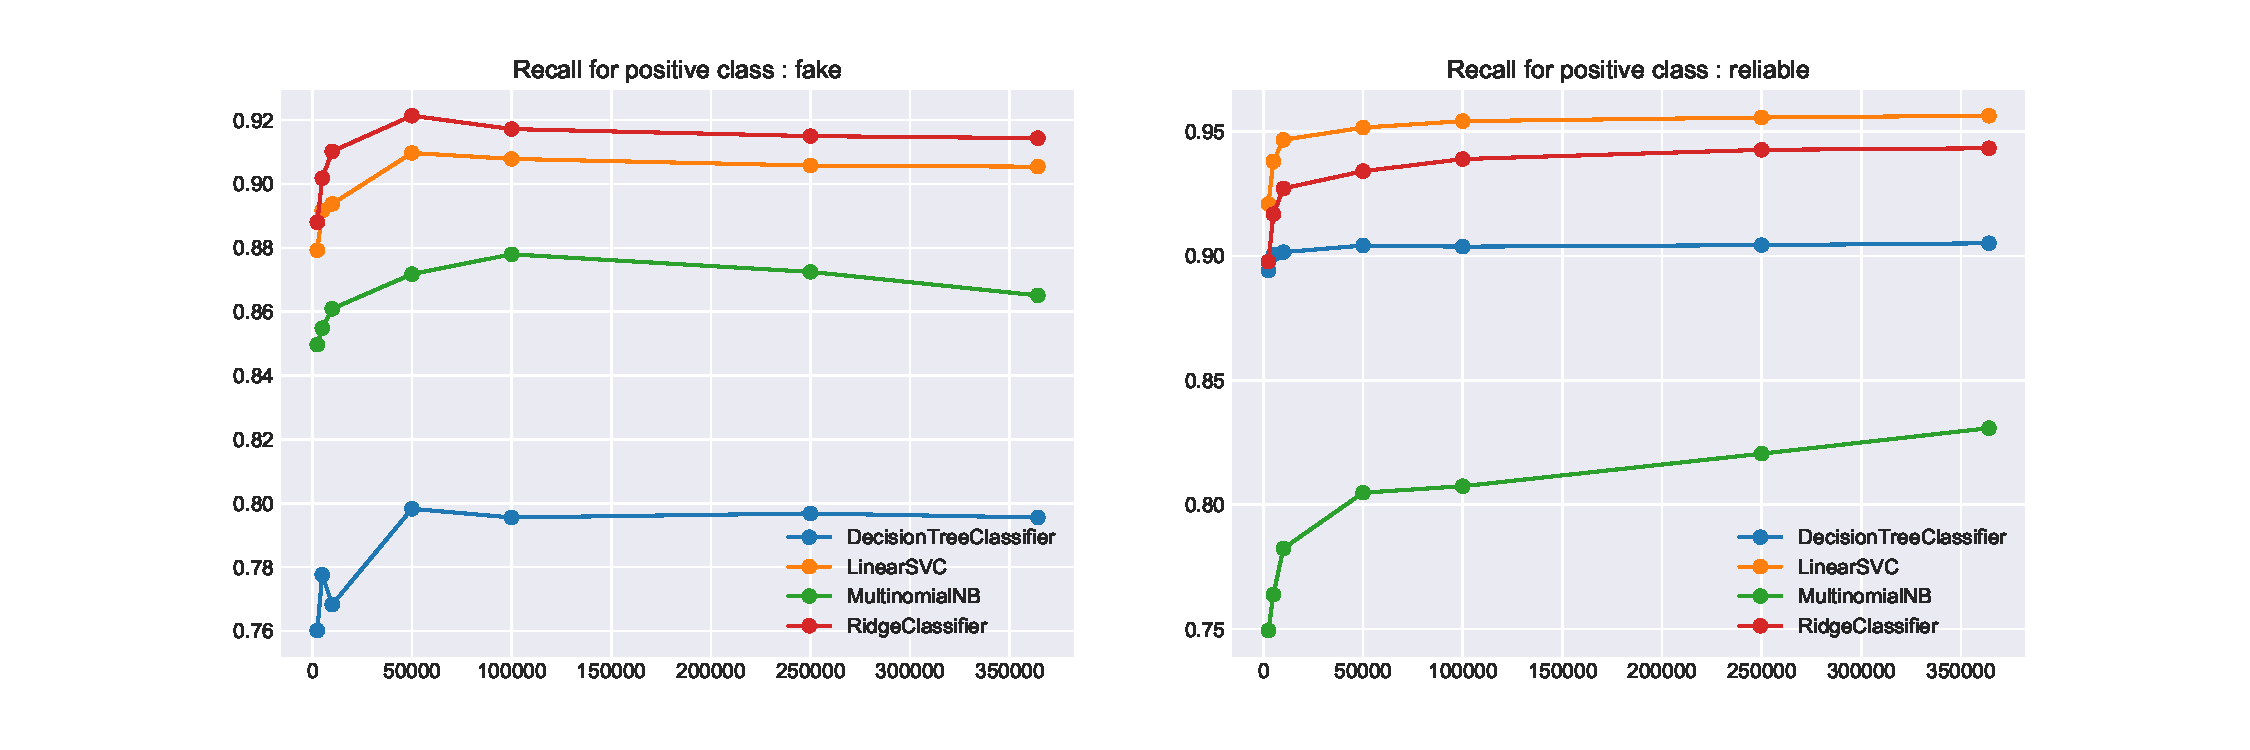
\includegraphics[width=0.8\textwidth]{images/chapitre3/ML_SMOTE_fake_recall}
 \caption{Recall for fake and reliable class for each model with respect to the maximum number of features}
 \label{fig:chap3:smote_max_feat3}
\end{figure*}
It conclusion for SMOTE method we can say that it does help models that do not have a regularization parameter or when the regularization parameter is low. Thus it does help prevent overfitting.
\section{Results on testing set}
\subsection{Methodology}
Now that all the models have been tuned, they need to be tested independently on testing set. Each dataset contains a testing set. \\
For the \textbf{liar-liar} dataset the following parameters will be used:
\begin{itemize}
 \item Linear SVM with regularization parameters of $0.1$ of a max TF-IDF features of 500,
 \item Ridge Classifier with $\alpha = 10$ and also max TF-IDF features of 500,
 \item Decision Tree with maximum depth of 1000 and the maximum number of features for TF-IDF,
 \item Na\"{i}ve-Bayes will also use the maximum number of features for TF-IDF.
\end{itemize}
For the \textbf{Fake News Corpus}, the following setting will be used:
\begin{itemize}
 \item Linear SVM with regularization parameters of $1$,
 \item Ridge Classifier with $\alpha = 1$,
 \item Decision Tree with maximum depth of 100.
\end{itemize}
They will all be trained using $100,000$ features for TF-IDF.
For the \textbf{Fake News Corpus} with SMOTE, the same parameters will be used, but the maximum number of features for TF-IDF will be used.\\
All the models will be trained on train and validation set and tested on test set. 
\subsection{Results}
\subsubsection{Liar-Liar Corpus}
By looking at the row results, based on average accuracy Na\"{i}ve-Bayes, Linear SVM and ridge classifiers perform very close, but when looking at the recall per class it shows that Na\"{i}ve-Bayes is bad at detecting fake news and classifies most of the text as reliable, when Linear SVM and Ridge classifiers are more balanced. 
\begin{table}
\begin{subtable}{\textwidth}
\begin{tabular}{lrrrrr}
\toprule
{} &         fake &     reliable &  accuracy &    macro avg &  weighted avg \\
\midrule
f1-score  &     0.514399 &     0.679764 &  0.614049 &     0.597082 &      0.607588 \\
precision &     0.570485 &     0.638376 &  0.614049 &     0.604430 &      0.608744 \\
recall    &     0.468354 &     0.726891 &  0.614049 &     0.597623 &      0.614049 \\
support   &  1106.000000 &  1428.000000 &  0.614049 &  2534.000000 &   2534.000000 \\
\bottomrule
\end{tabular}
\caption{Raw results for Linear SVM}
\end{subtable}
\begin{subtable}{\textwidth}
\begin{tabular}{lrrrrr}
\toprule
{} &         fake &     reliable &  accuracy &    macro avg &  weighted avg \\
\midrule
f1-score  &     0.412107 &     0.698507 &  0.601421 &     0.555307 &      0.573504 \\
precision &     0.578431 &     0.608741 &  0.601421 &     0.593586 &      0.595512 \\
recall    &     0.320072 &     0.819328 &  0.601421 &     0.569700 &      0.601421 \\
support   &  1106.000000 &  1428.000000 &  0.601421 &  2534.000000 &   2534.000000 \\
\bottomrule
\end{tabular}
\caption{Raw results for Na\"{i}ve-Bayes}
\end{subtable}
\begin{subtable}{\textwidth}
\begin{tabular}{lrrrrr}
\toprule
{} &         fake &     reliable &  accuracy &    macro avg &  weighted avg \\
\midrule
f1-score  &     0.496366 &     0.691279 &  0.617206 &     0.593822 &      0.606207 \\
precision &     0.582927 &     0.633606 &  0.617206 &     0.608266 &      0.611486 \\
recall    &     0.432188 &     0.760504 &  0.617206 &     0.596346 &      0.617206 \\
support   &  1106.000000 &  1428.000000 &  0.617206 &  2534.000000 &   2534.000000 \\
\bottomrule
\end{tabular}
\caption{Raw results for Ridge Classifer.}
\end{subtable}
\begin{subtable}{\textwidth}
\begin{tabular}{lrrrrr}
\toprule
{} &         fake &     reliable &  accuracy &    macro avg &  weighted avg \\
\midrule
f1-score  &     0.479354 &     0.591549 &  0.542226 &     0.535451 &      0.542580 \\
precision &     0.475936 &     0.594901 &  0.542226 &     0.535418 &      0.542977 \\
recall    &     0.482821 &     0.588235 &  0.542226 &     0.535528 &      0.542226 \\
support   &  1106.000000 &  1428.000000 &  0.542226 &  2534.000000 &   2534.000000 \\
\bottomrule
\end{tabular}
\caption{Raw results for Decision Tree}
\end{subtable}
\caption{Raw results on \textbf{Liar-Liar Corpus}.}
\end{table}
Finally, it is possible to look at the ROC curve at \textbf{Figure \ref{fig:chap3:roc1}}. One more time, it shows that Na\"{i}ve-Bayes, linear svm and ridge classifier have similar performance, but in this case it shows that NB has a little advantage, with a slightly larger AUC. There is only one point for the decision tree as it does not output probabilities for each class. \\
\begin{figure*}
 \centering
 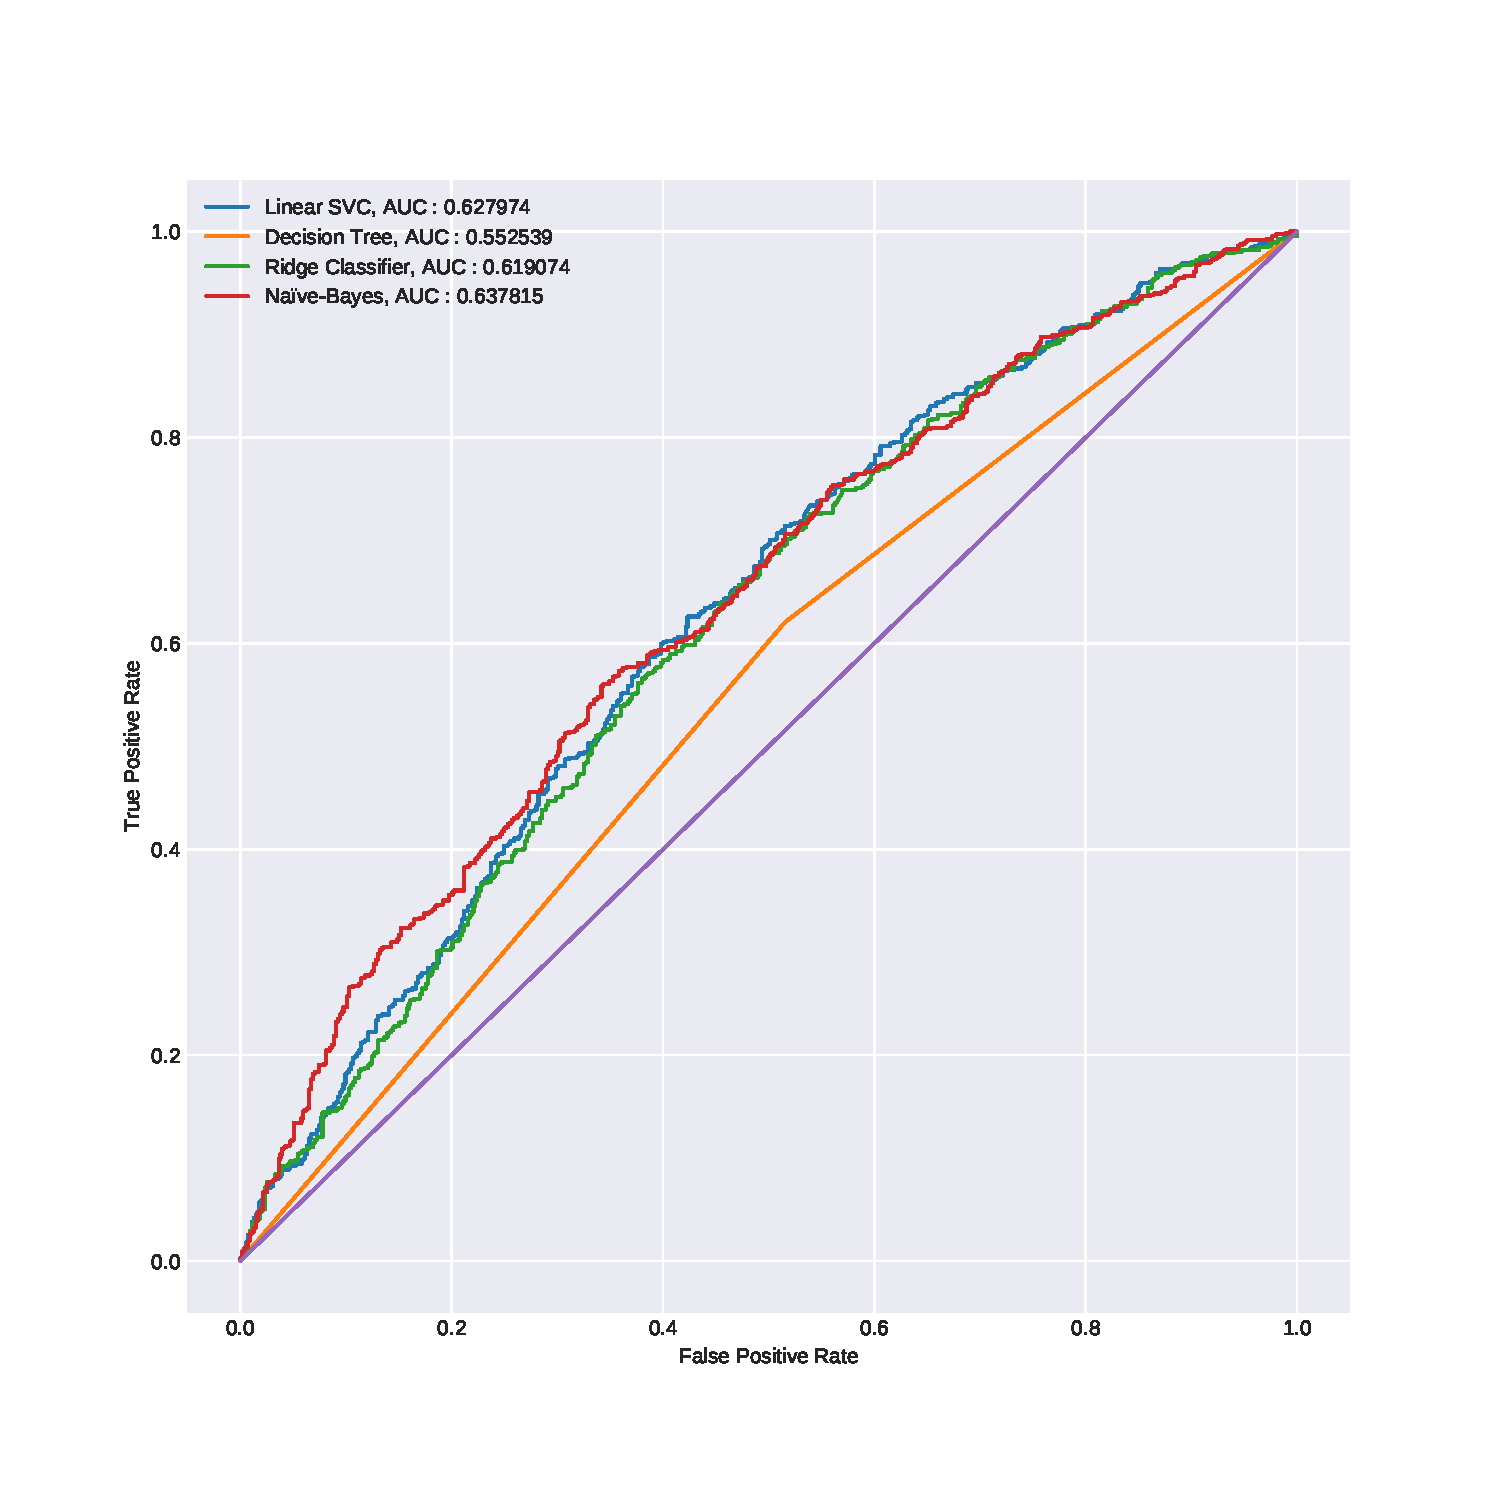
\includegraphics[width=0.8\textwidth]{images/chapitre3/roc1}
 \caption{ROC curve for each model}
 \label{fig:chap3:roc1}
\end{figure*}
\begin{figure*}
 \centering
 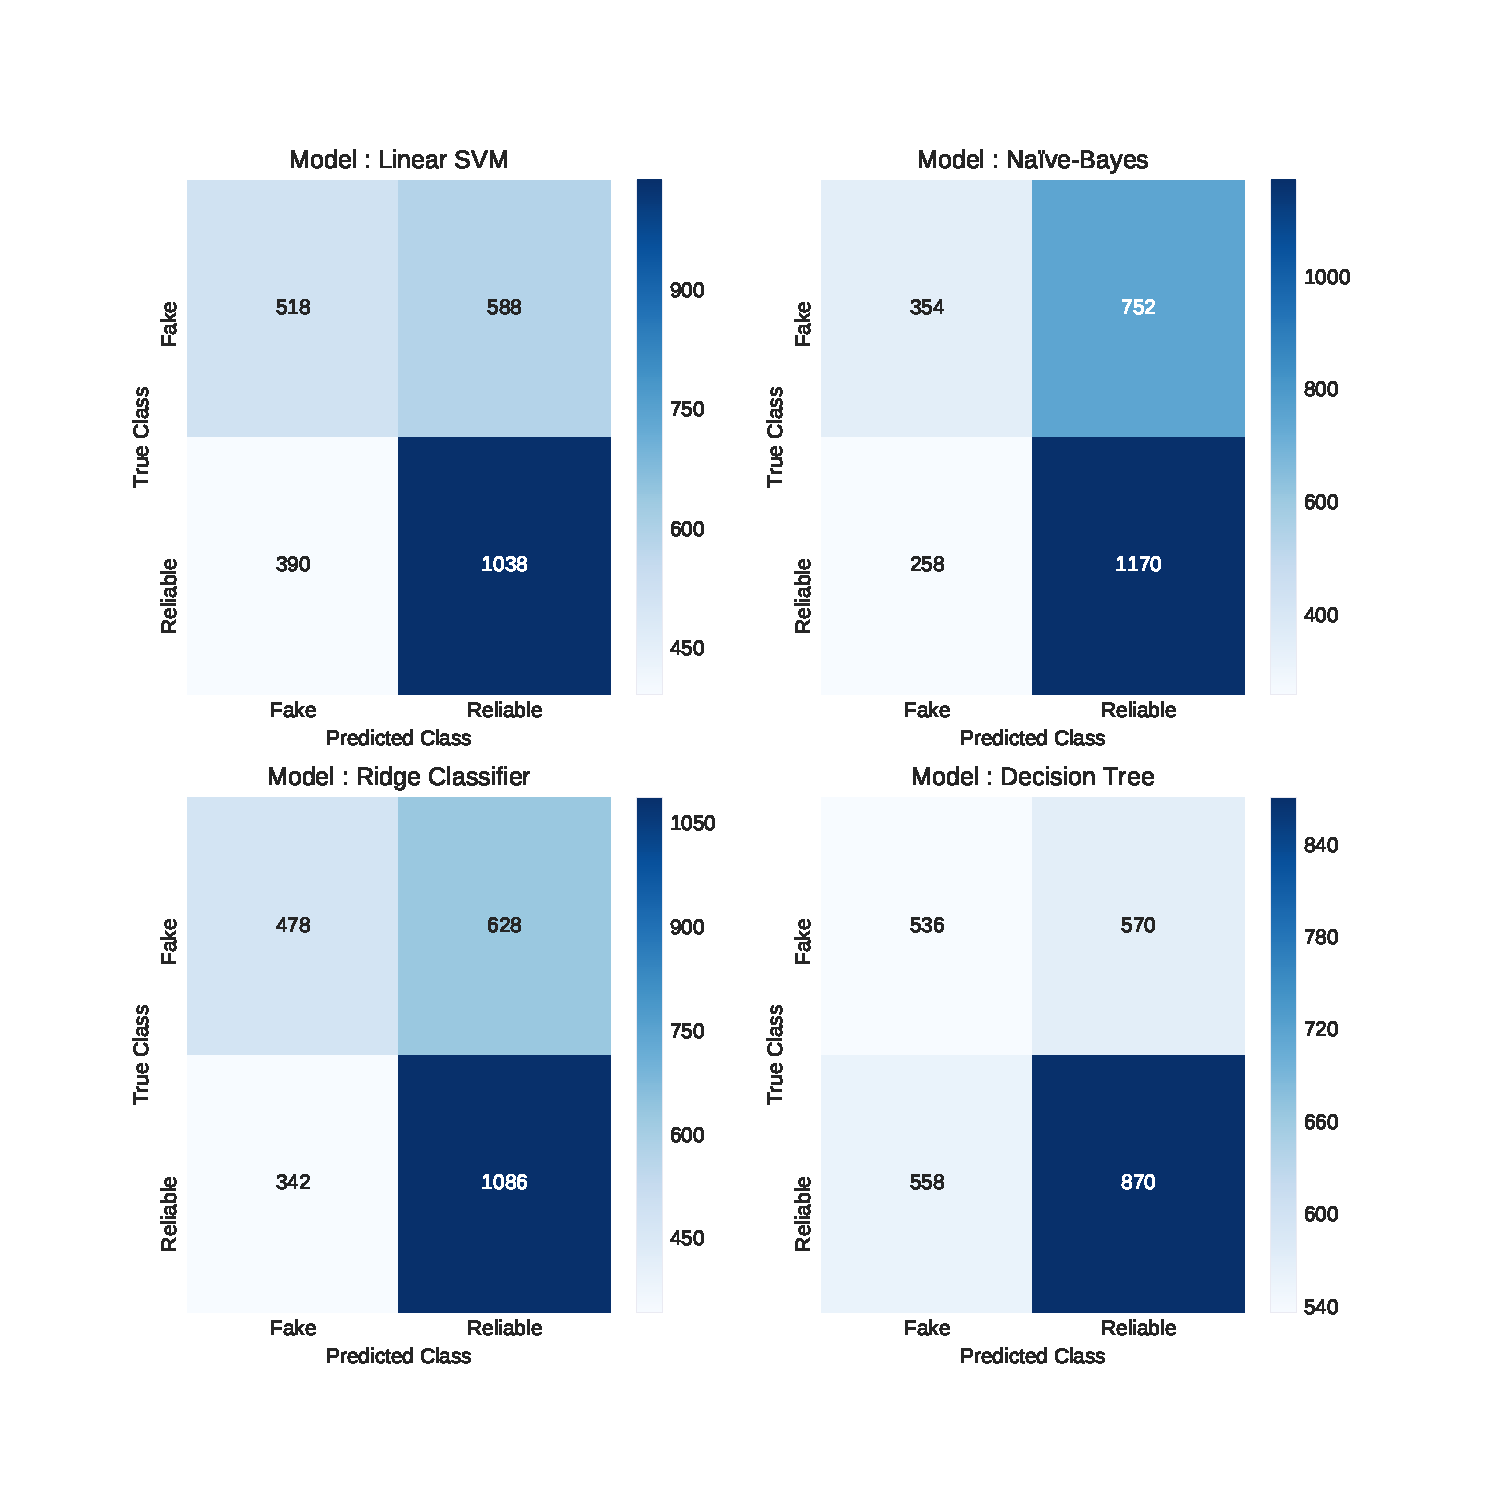
\includegraphics[width=0.8\textwidth]{images/chapitre3/test_liar_confMat}
 \caption{Confusion Matrix for each models}
 \label{fig:chap3:confMat1}
\end{figure*}
When it comes to the \textbf{Fake news corpus}, linear models are still the ones that perform the best, with linear svm reaching an accuracy of $94.7\%$ and ridge classifiers $93.98\%$. Surprisingly, decision tree outperform Na\"{i}ve-Bayes in this case, with an accuracy of $89.4\%$ when Na\"{i}ve-Bayes only gets $85.3\%$.\\
\begin{table}
\begin{subtable}{\textwidth}
 \begin{tabular}{lrrrrr}
 \toprule
 {} &          fake &      reliable &  accuracy &     macro avg &  weighted avg \\
 \midrule
 f1-score  &      0.894700 &      0.965364 &  0.947874 &      0.930032 &      0.947620 \\
 precision &      0.907861 &      0.960783 &  0.947874 &      0.934322 &      0.947494 \\
 recall    &      0.881916 &      0.969989 &  0.947874 &      0.925952 &      0.947874 \\
 support   &  17496.000000 &  52181.000000 &  0.947874 &  69677.000000 &  69677.000000 \\
 \bottomrule
 \end{tabular}
 \caption{Raw results for Linear SVM on \textbf{Fake News Corpus}}
\end{subtable}
\begin{subtable}{\textwidth}
 \begin{tabular}{lrrrrr}
 \toprule
 {} &          fake &      reliable &  accuracy &     macro avg &  weighted avg \\
 \midrule
 f1-score  &      0.674458 &      0.905634 &  0.853682 &      0.790046 &      0.847585 \\
 precision &      0.764127 &      0.875841 &  0.853682 &      0.819984 &      0.847790 \\
 recall    &      0.603624 &      0.937525 &  0.853682 &      0.770574 &      0.853682 \\
 support   &  17496.000000 &  52181.000000 &  0.853682 &  69677.000000 &  69677.000000 \\
 \bottomrule
 \end{tabular}
 \caption{Raw results for Na\"{i}ve-Bayes on \textbf{Fake News Corpus}}
\end{subtable}
\begin{subtable}{\textwidth}
 \begin{tabular}{lrrrrr}
 \toprule
 {} &          fake &      reliable &  accuracy &     macro avg &  weighted avg \\
 \midrule
 f1-score  &      0.874220 &      0.960438 &  0.939808 &      0.917329 &      0.938788 \\
 precision &      0.919674 &      0.945736 &  0.939808 &      0.932705 &      0.939192 \\
 recall    &      0.833048 &      0.975604 &  0.939808 &      0.904326 &      0.939808 \\
 support   &  17496.000000 &  52181.000000 &  0.939808 &  69677.000000 &  69677.000000 \\
 \bottomrule
 \end{tabular}
 \caption{Raw results for Ridge Classifier on \textbf{Fake News Corpus}}
\end{subtable}
\begin{subtable}{\textwidth}
 \begin{tabular}{lrrrrr}
 \toprule
 {} &          fake &      reliable &  accuracy &     macro avg &  weighted avg \\
 \midrule
 f1-score  &      0.791687 &      0.929799 &  0.894987 &      0.860743 &      0.895119 \\
 precision &      0.788700 &      0.930987 &  0.894987 &      0.859844 &      0.895258 \\
 recall    &      0.794696 &      0.928614 &  0.894987 &      0.861655 &      0.894987 \\
 support   &  17496.000000 &  52181.000000 &  0.894987 &  69677.000000 &  69677.000000 \\
 \bottomrule
 \end{tabular}
 \caption{Raw results for Decision Tree on \textbf{Fake News Corpus}}
\end{subtable}
\caption{Results on \textbf{Fake News Corpus} without using SMOTE.}
\end{table}
In this case, the ROC curve (\textbf{Figure \ref{fig:chap3:roc2}}) shows almost the same ranking of models, except for Decision Tree that is the last one, and Na\"{i}ve-Bayes being juste above it. 
\begin{figure*}
 \centering
 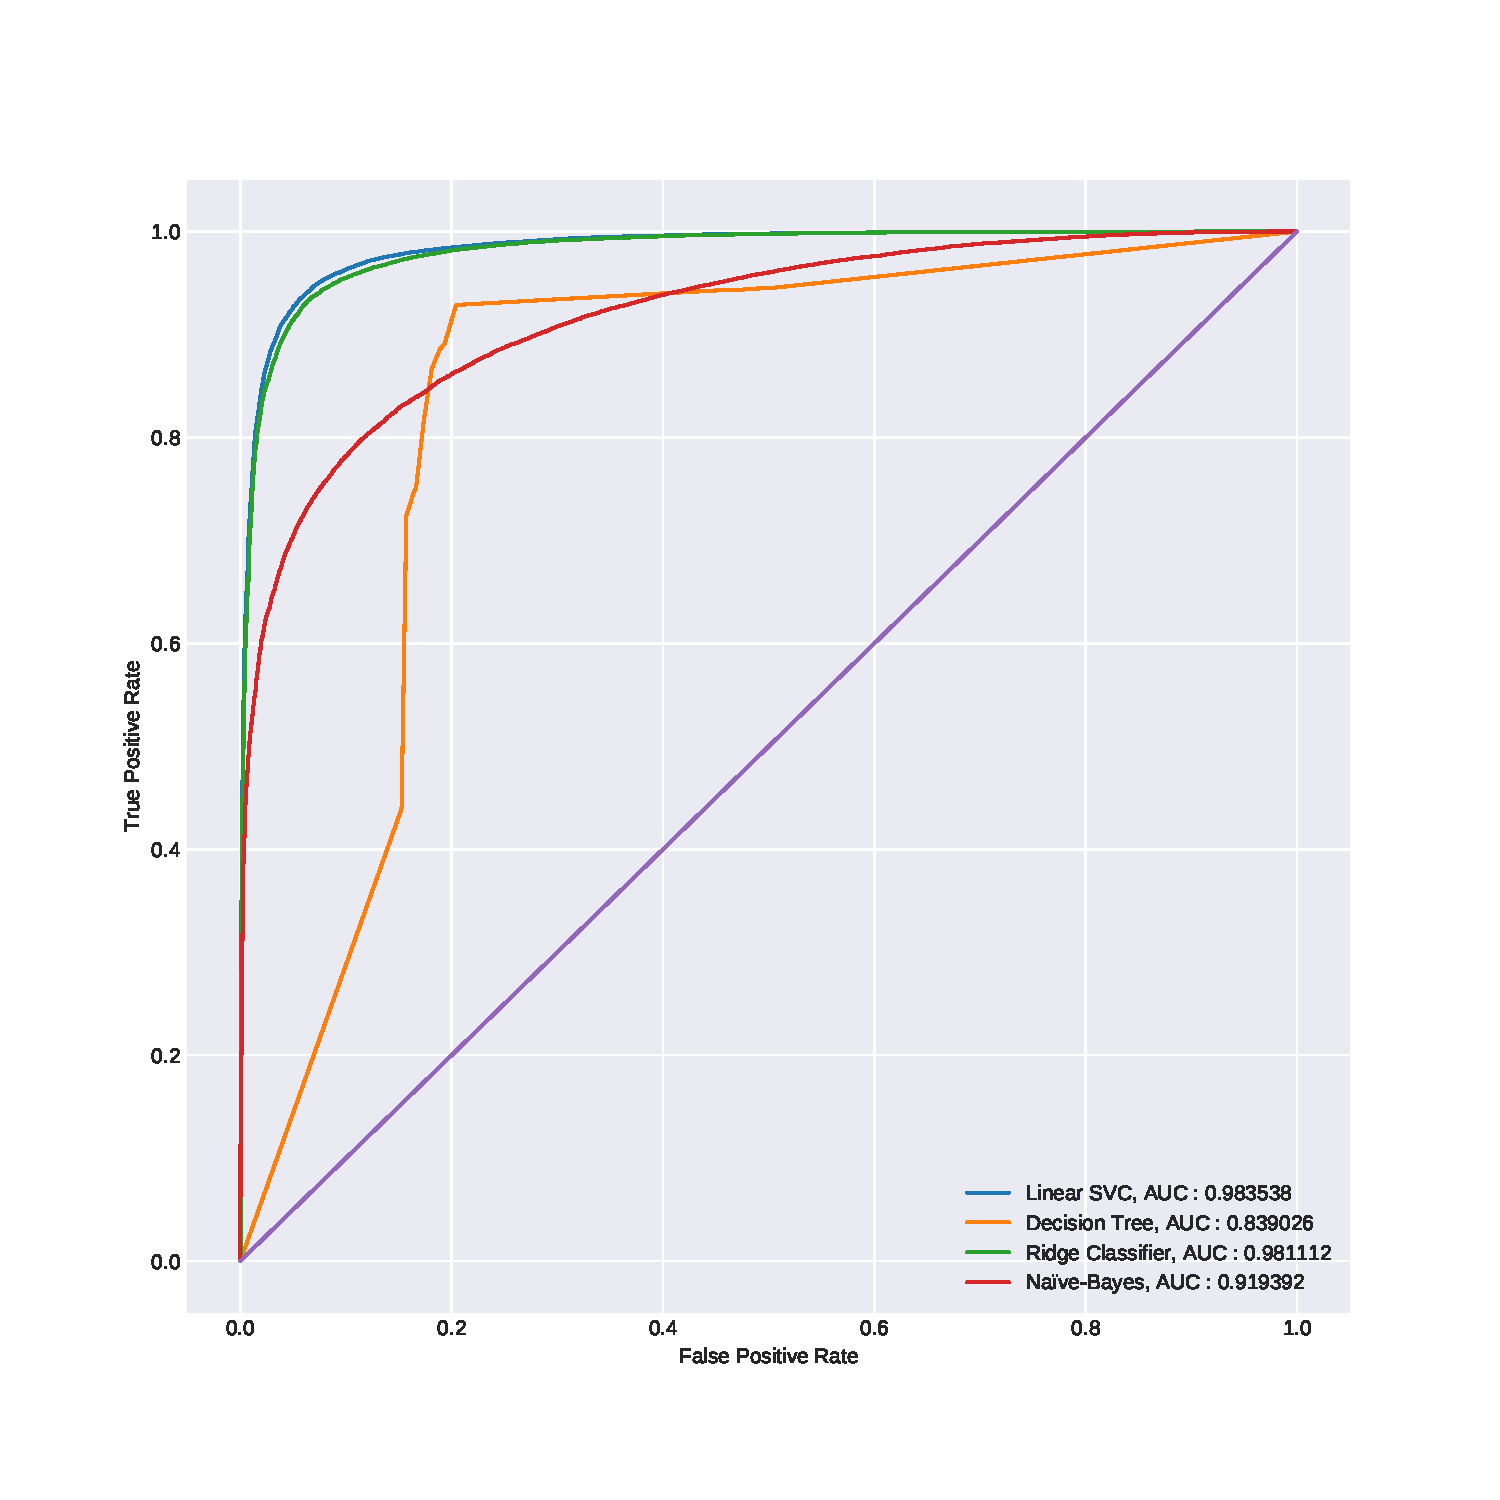
\includegraphics[width=0.8\textwidth]{images/chapitre3/roc2}
 \caption{ROC curve for each model}
 \label{fig:chap3:roc2}
\end{figure*}
Confusion matrix (\textbf{Figure \ref{fig:chap3:confMat2}}) shows that Na\"{i}ve-Bayes has a tendency of classifying fake news as being reliable. And the other hand, ridge classifier is the one that makes the least misclassification for reliable news, which is a good point. \\
\begin{figure*}
 \centering
 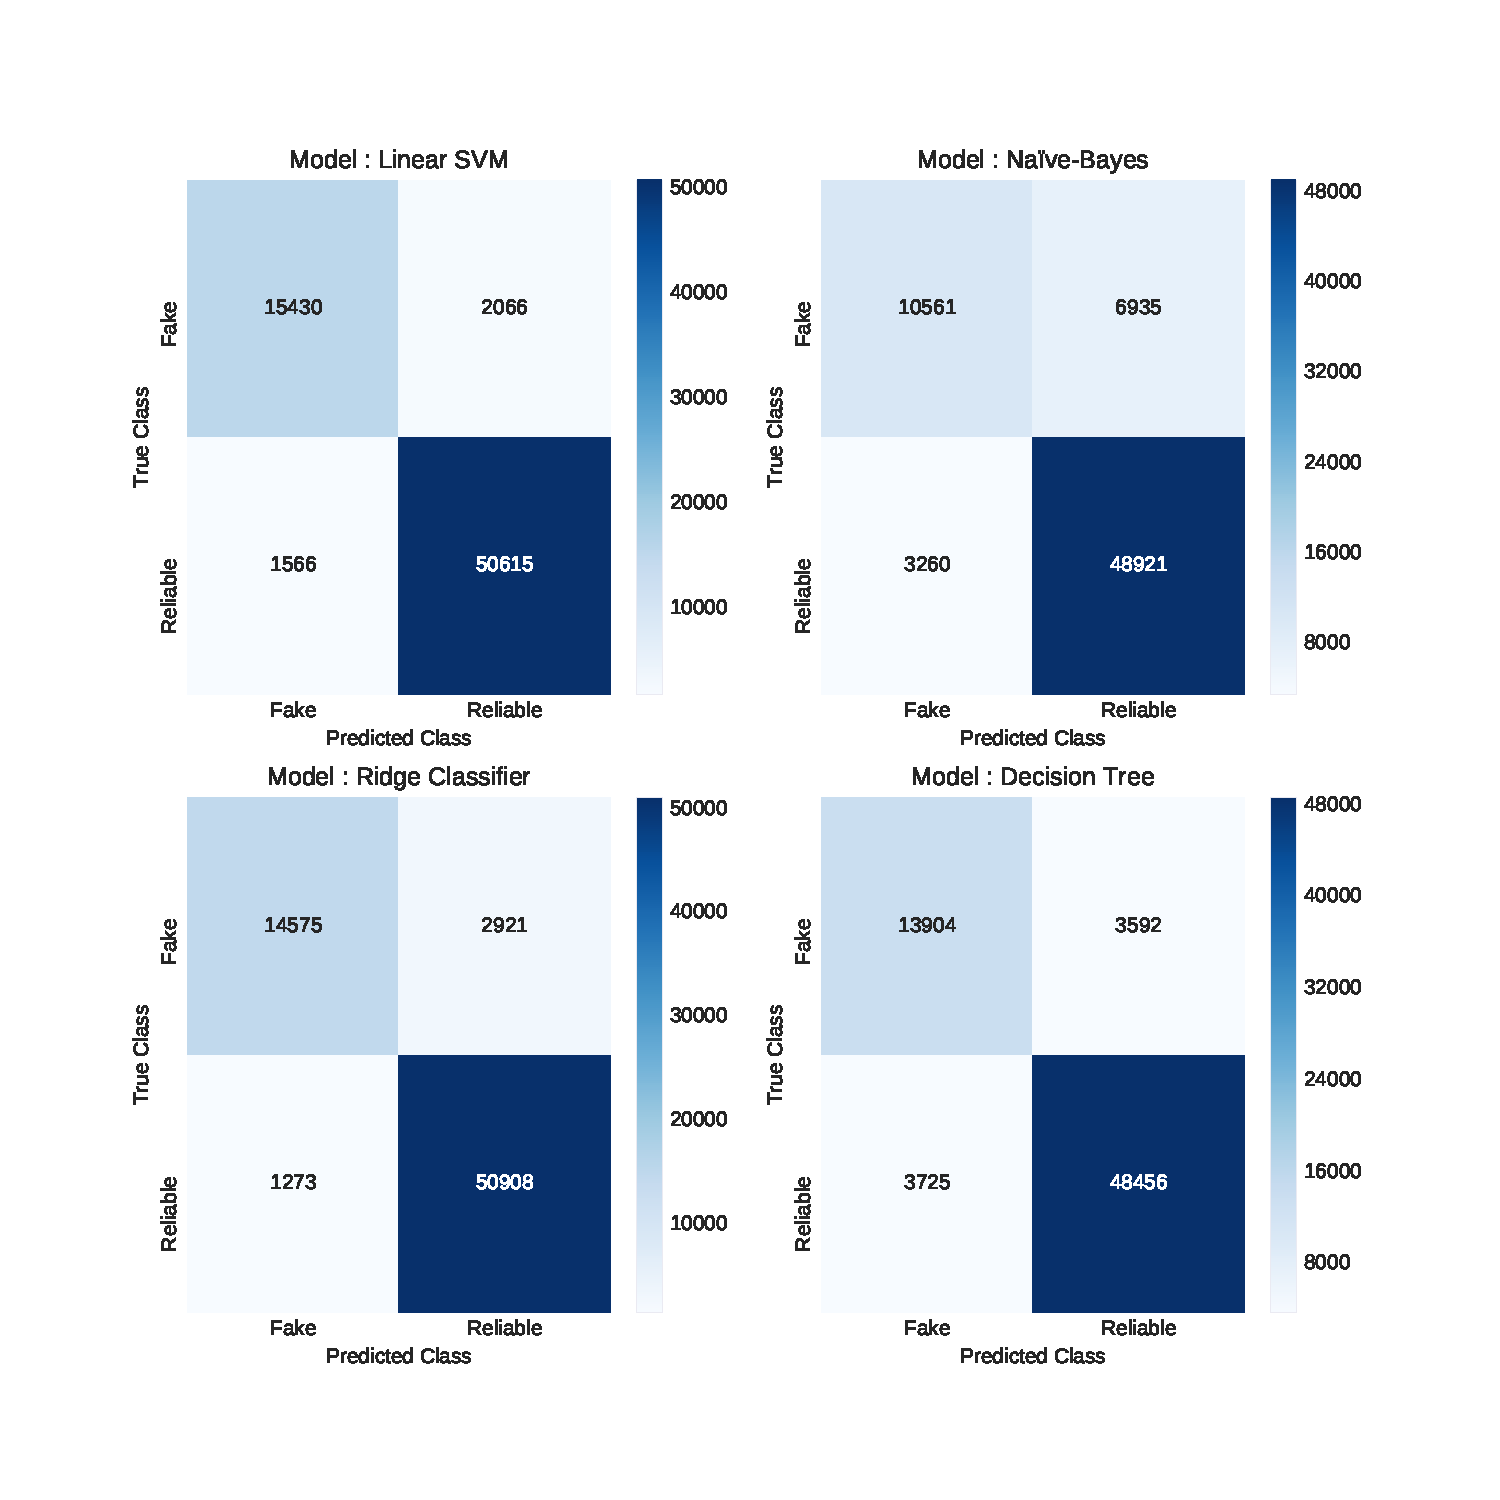
\includegraphics[width=0.8\textwidth]{images/chapitre3/test_fake_confMat}
 \caption{Confusion Matrix for Each models}
 \label{fig:chap3:confMat2}
\end{figure*}
Finally, there is the results of the models trained with SMOTE data augmentation. Using it shows little to no improvements. The only benefit is to balance a little bit the recall for Na\"{i}ve-Bayes on fake and reliable news. 
\begin{table}
\begin{subtable}{\textwidth}
 \begin{tabular}{lrrrrr}
 \toprule
 {} &          fake &      reliable &  accuracy &     macro avg &  weighted avg \\
 \midrule
 f1-score  &      0.891373 &      0.962340 &   0.94407 &      0.926857 &      0.944520 \\
 precision &      0.869960 &      0.970623 &   0.94407 &      0.920291 &      0.945346 \\
 recall    &      0.913866 &      0.954198 &   0.94407 &      0.934032 &      0.944070 \\
 support   &  17496.000000 &  52181.000000 &   0.94407 &  69677.000000 &  69677.000000 \\
 \bottomrule
 \end{tabular}
 \caption{Raw results of linear svm on \textbf{Fake News Corpus} when training using SMOTE}
\end{subtable}
\begin{subtable}{\textwidth}
 \begin{tabular}{lrrrrr}
 \toprule
 {} &          fake &      reliable &  accuracy &     macro avg &  weighted avg \\
 \midrule
 f1-score  &      0.714816 &      0.873538 &  0.824777 &      0.794177 &      0.833683 \\
 precision &      0.604424 &      0.950521 &  0.824777 &      0.777472 &      0.863615 \\
 recall    &      0.874543 &      0.808091 &  0.824777 &      0.841317 &      0.824777 \\
 support   &  17496.000000 &  52181.000000 &  0.824777 &  69677.000000 &  69677.000000 \\
 \bottomrule
 \end{tabular}
 \caption{Raw results of Na\"{i}ve-Bayes on \textbf{Fake News Corpus} when training using SMOTE}
\end{subtable}
\begin{subtable}{\textwidth}
 \begin{tabular}{lrrrrr}
 \toprule
 {} &          fake &      reliable &  accuracy &     macro avg &  weighted avg \\
 \midrule
 f1-score  &      0.877755 &      0.956129 &  0.935431 &      0.916942 &      0.936449 \\
 precision &      0.836588 &      0.973317 &  0.935431 &      0.904953 &      0.938984 \\
 recall    &      0.923182 &      0.939537 &  0.935431 &      0.931360 &      0.935431 \\
 support   &  17496.000000 &  52181.000000 &  0.935431 &  69677.000000 &  69677.000000 \\
 \bottomrule
 \end{tabular}
 \caption{Raw results of Ridge Classifier on \textbf{Fake News Corpus} when training using SMOTE}
\end{subtable}
\begin{subtable}{\textwidth}
 \begin{tabular}{lrrrrr}
 \toprule
 {} &          fake &      reliable &  accuracy &     macro avg &  weighted avg \\
 \midrule
 f1-score  &      0.787226 &      0.921178 &  0.884969 &      0.854202 &      0.887542 \\
 precision &      0.734992 &      0.946085 &  0.884969 &      0.840539 &      0.893079 \\
 recall    &      0.847451 &      0.897549 &  0.884969 &      0.872500 &      0.884969 \\
 support   &  17496.000000 &  52181.000000 &  0.884969 &  69677.000000 &  69677.000000 \\
 \bottomrule
 \end{tabular}
 \caption{Raw results of Decision tree on \textbf{Fake News Corpus} when training using SMOTE}
\end{subtable}
\caption{Results on \textbf{Fake News Corpus} when training with SMOTE.}
\end{table}
\begin{figure*}
 \centering
 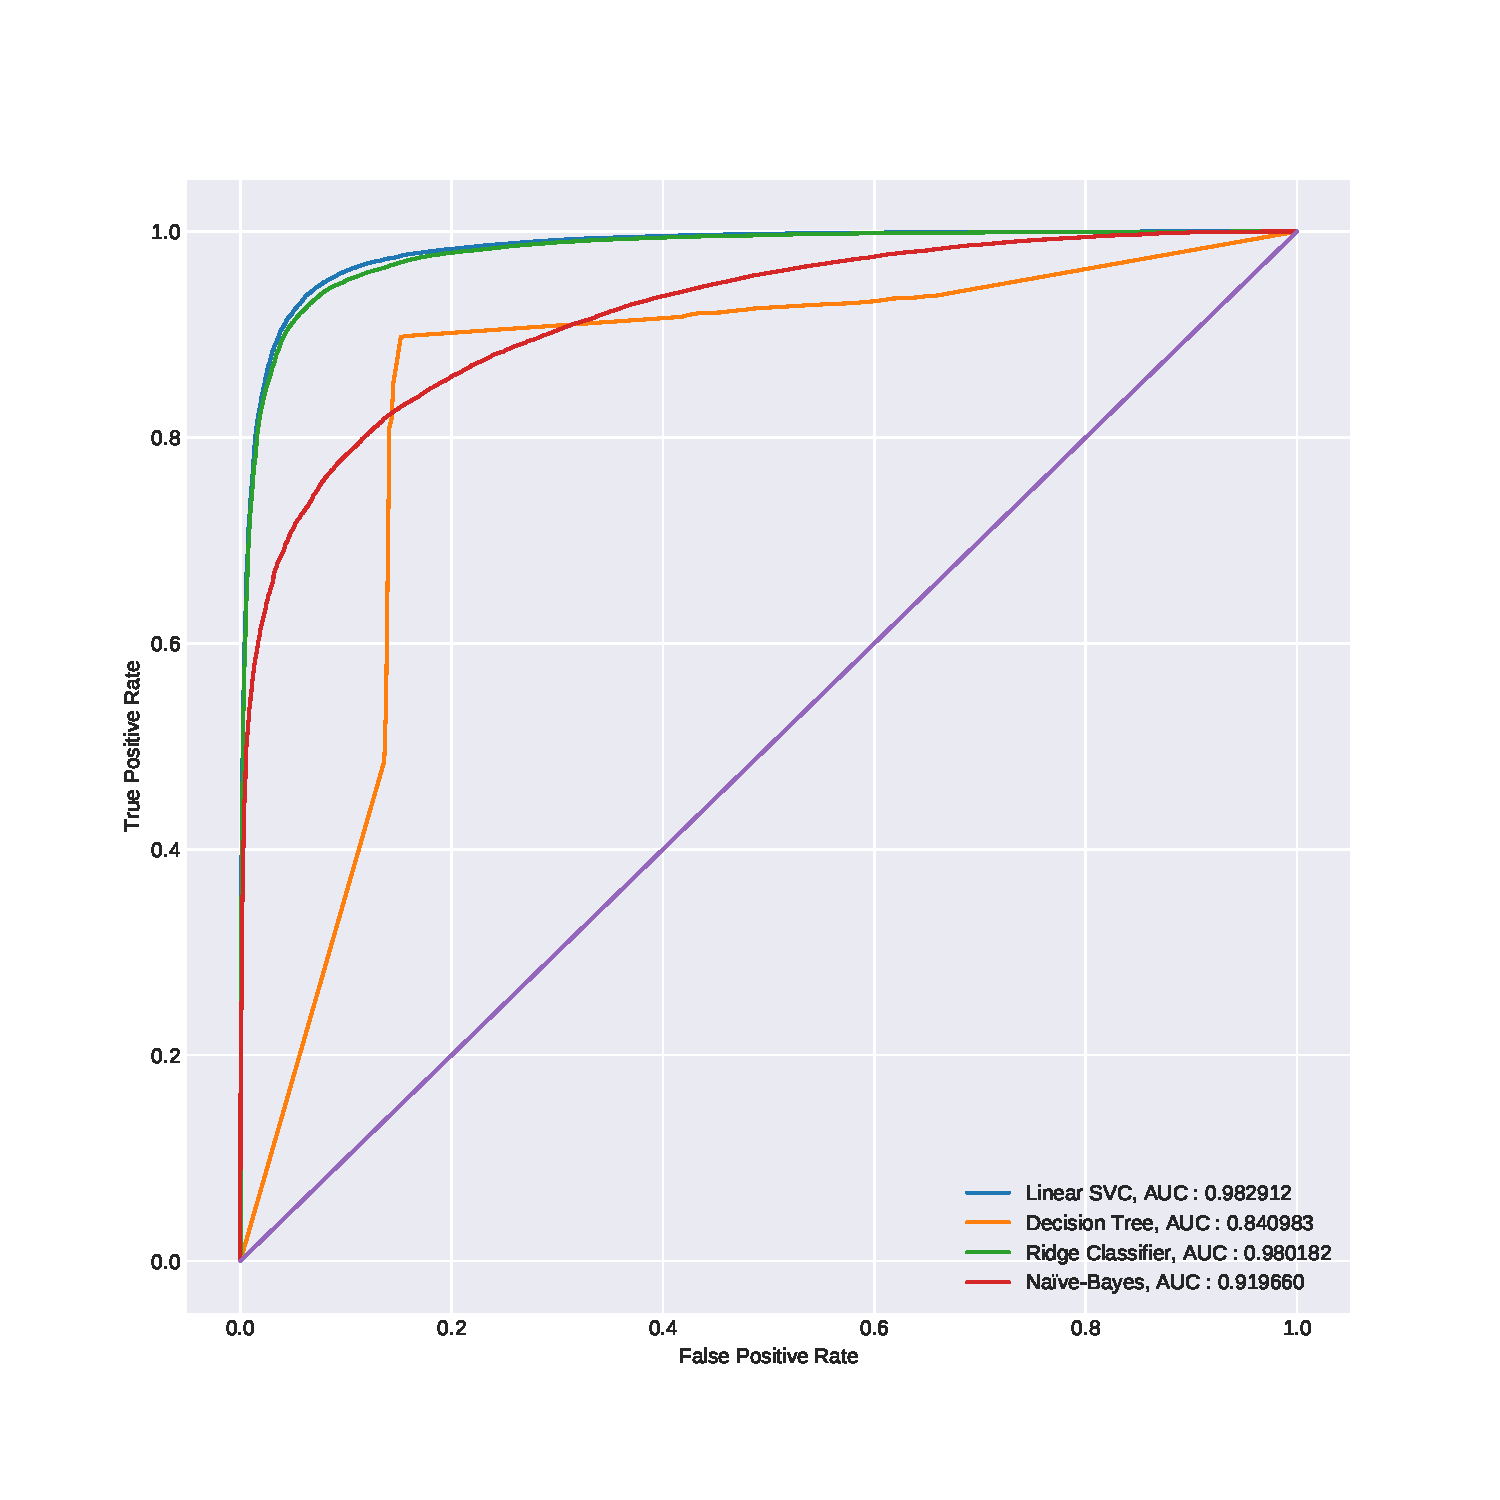
\includegraphics[width=0.8\textwidth]{images/chapitre3/roc3}
 \caption{ROC curve for each model}
 \label{fig:chap3:roc3}
\end{figure*}
\begin{figure*}
 \centering
 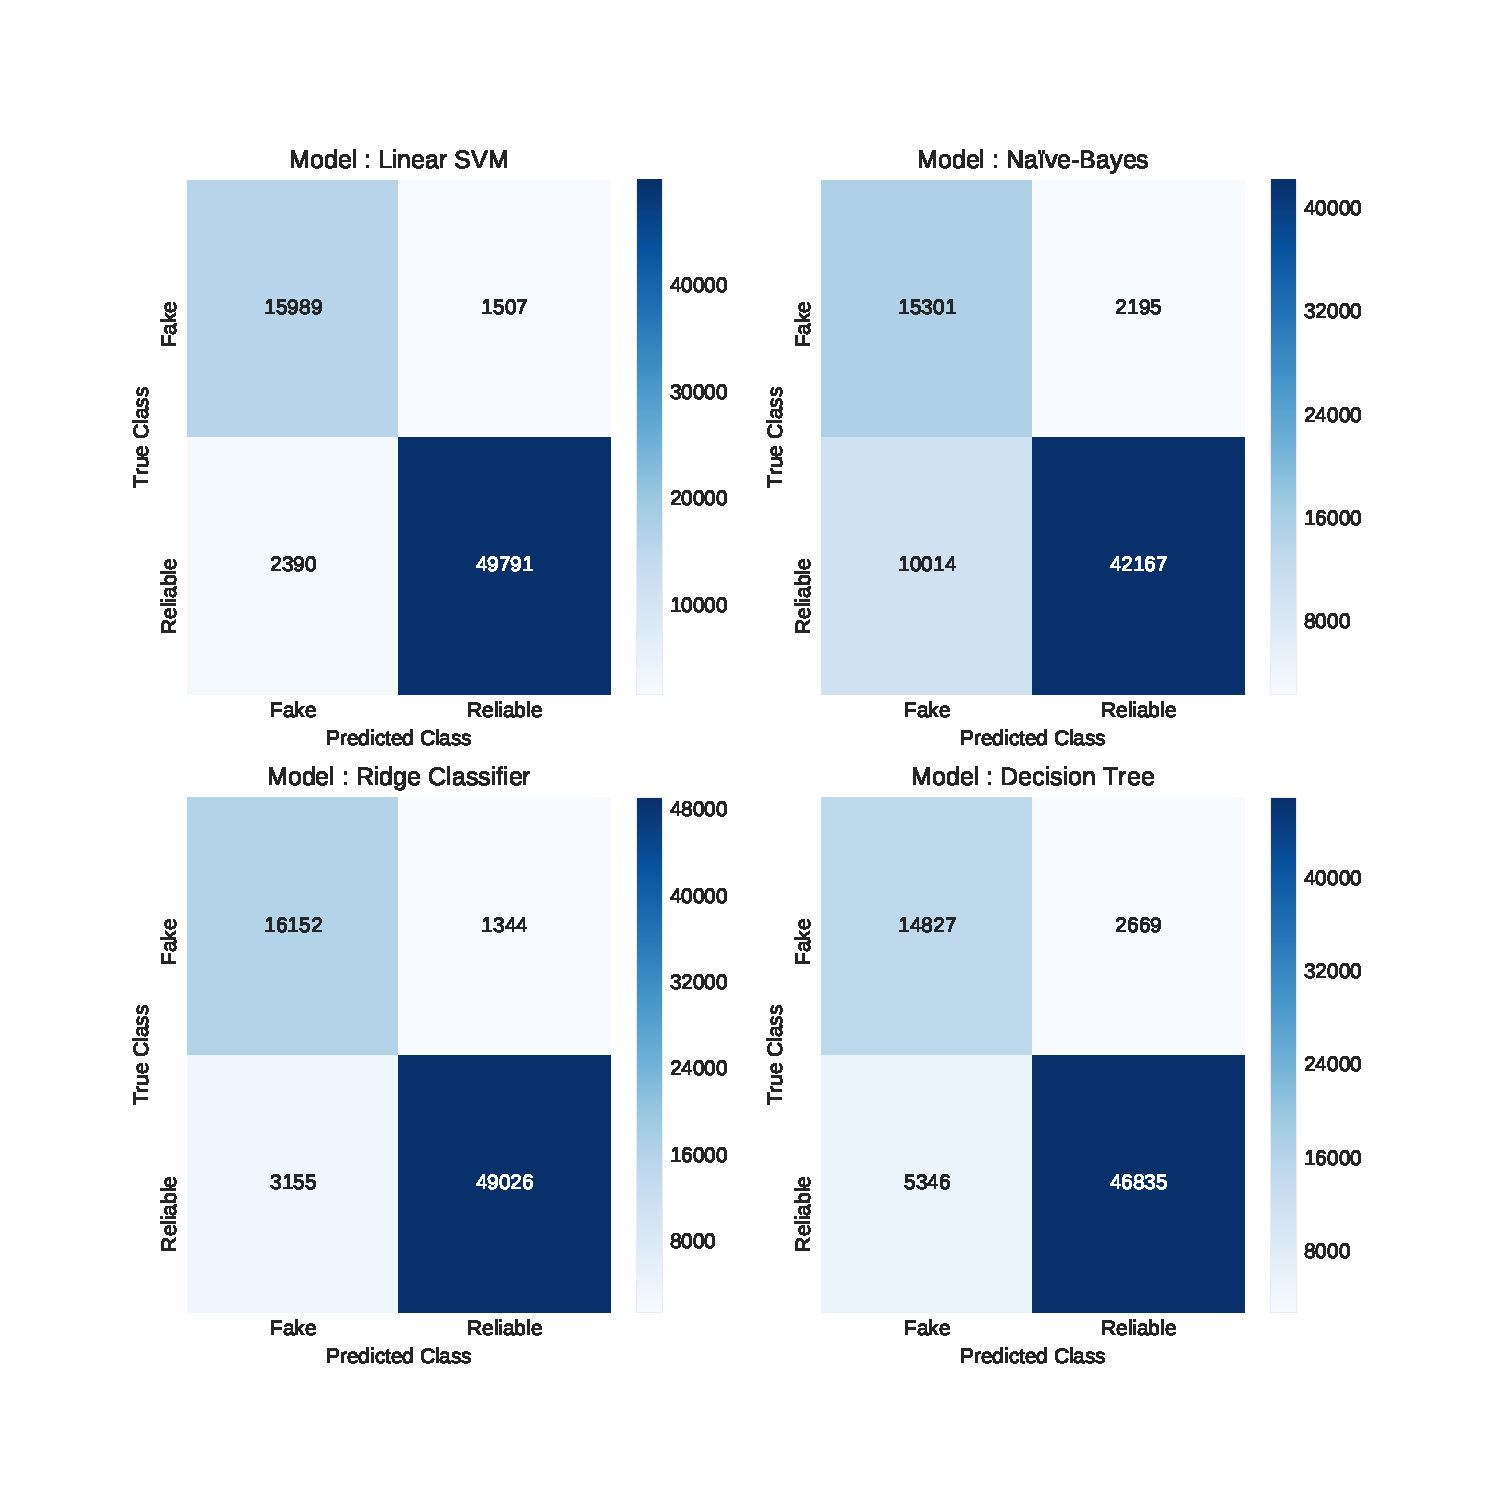
\includegraphics[width=0.8\textwidth]{images/chapitre3/test_SMOTE_fake_confMat}
 \caption{Confusion Matrix for each models}
 \label{fig:chap3:confMat3}
\end{figure*}
\section{Conclusion}
In this chapter we have analysed how traditional machine learning algorithms words on two different datasets, the second being imbalanced a data augmentation technique, called SMOTE, has been used in order to see if it improves the results. \\
We can conclude that in all the cases linear models are the ones that work the best, with a top accuracy of $61.7\%$ on the \textbf{liar-liar corpus} using Ridge Classifier, and a top accuracy of $94.7\%$ on the \textbf{Fake News Corpus} using linear svm. At the end, the result obtains on the second data set are really good, when those obtain on the first when are mitigated. \\
As explained earlier, it might be important to choose to model that makes the smaller misclassification rate on reliable news in order to avoid possible censorship and confusion matrix shows that in both case Ridge Classifiers is the ones that make the fewer errors in that case. \\
In addition, we have shown that Synthectic Minority Over Sampling Techniques acts as a regularizers, as it does improve performance when the penalization term in small on linear models. \\
In the next section, the focus will be put on trying to improve results on the \textbf{Liar-Liar corpus} as there is room for improvement and that the second dataset already as very good results. But models will still be trying on it for comparison. 